\documentclass[a4paper,12pt]{article}
\usepackage[utf8]{inputenc}
\usepackage[german]{babel}
\usepackage{amsmath}
\usepackage{amssymb}
\usepackage{amsthm}
\usepackage{geometry}
\usepackage{graphicx}
\usepackage[hidelinks]{hyperref}
\usepackage{listings}
\usepackage{xcolor}
\usepackage{microtype}
\usepackage{enumitem}
\usepackage{tikz}
\usepackage{pgfplots}
\pgfplotsset{compat=1.18}
\usetikzlibrary{arrows.meta, positioning, shapes.geometric, fit, calc}
\usepackage{booktabs}
\usepackage{caption}
\usepackage{subcaption}
\usepackage{float}

\geometry{margin=2.5cm}

\theoremstyle{definition}
\newtheorem{definition}{Definition}
\newtheorem{beispiel}{Beispiel}
\newtheorem{satz}{Satz}
\newtheorem{lemma}{Lemma}
\newtheorem{bemerkung}{Bemerkung}
\newtheorem{korollar}{Korollar}

\setlist[itemize,1]{label=--}

% ---------- Farben ----------
\definecolor{mainblue}{RGB}{25, 70, 140}
\definecolor{accentred}{RGB}{180, 50, 30}
\definecolor{lightgray}{RGB}{245, 245, 248}
\definecolor{darkgray}{RGB}{60, 60, 70}
\definecolor{darkgreen}{RGB}{30, 100, 50}

\hypersetup{
    colorlinks=true,
    linkcolor=mainblue,
    citecolor=accentred,
    urlcolor=mainblue,
    pdftitle={Zentrales Reifendruckregelsystem: Formale Analyse, Verschleißoptimierung und Systemarchitektur},
    pdfauthor={Stephan Epp},
}

% Code-Highlighting
\lstset{
    basicstyle=\ttfamily\small,
    keywordstyle=\color{blue},
    commentstyle=\color{gray},
    stringstyle=\color{accentred},
    numbers=left,
    numberstyle=\tiny,
    breaklines=true,
    frame=single,
    backgroundcolor=\color{lightgray},
    literate=%
    {Ö}{{\"O}}1
    {Ä}{{\"A}}1
    {Ü}{{\"U}}1
    {ß}{{\ss}}1
    {ü}{{\"u}}1
    {ä}{{\"a}}1
    {ö}{{\"o}}1
    {<=}{{\texttt{<=}}}2
    {>=}{{\texttt{>=}}}2
}

\title{%
  \textbf{Zentrales Reifendruckregelsystem (ZRRS)}\\[0.4em]
  \large Formale Analyse, Verschleißoptimierung und Systemarchitektur\\
  für einöffnungsbasierte Druckluftversorgung in Kraftfahrzeugen
}
\author{Stephan Epp}
\date{29. März 2026}

\begin{document}

\maketitle

\tableofcontents
\newpage

% =============================================================================
\section{Einführung}
% =============================================================================
Das Zentralisierte Reifendruckregelsystem (ZRRS) adressiert eine grundlegende
Schwäche konventioneller Fahrzeugkonzepte: Die getrennte, manuelle Befüllung
jedes der vier Reifen führt zu systematischen Druckungleichgewichten, erhöhtem
und inhomogenem Reifenverschleiß sowie Sicherheitsrisiken durch Unterdruck.
Diese Arbeit stellt ein Systemkonzept vor, bei dem \emph{eine einzige
	Druckluftzuführungsöffnung} am Fahrzeug genügt; ein integriertes Steuergerät
verteilt den Luftdruck automatisch und gleichmäßig auf alle vier Räder.
Wir liefern formale Definitionen, Theorem-Beweis-Paare sowie empirisch
gestützte Simulationsergebnisse (matplotlib), die belegen, dass das ZRRS
den Reifenverschleiß um $\geq 18\,\%$ reduziert, die Druckstandardabweichung
von $\sigma_{\text{man}} = 0{,}15\,\text{bar}$ auf
$\sigma_{\text{ZRRS}} \leq 0{,}025\,\text{bar}$ senkt und die
Nutzerzuverlässigkeit gegenüber manuellem Befüllen signifikant steigert.

Reifendruck gehört zu den sicherheitsrelevantesten Fahrzeugparametern.
Studien des Kraftfahrt-Bundesamtes und der NHTSA zeigen, dass mehr als
$30\,\%$ aller Personenkraftwagen im normalen Straßenbetrieb mindestens einen
Reifen aufweisen, der mehr als $0{,}2\,\text{bar}$ unterhalb des Solldrucks
liegt \cite{nhtsa2001}. Die Konsequenzen sind vielfältig:

\begin{itemize}
    \item erhöhter und inhomogener Reifenabrieb an allen vier Rädern,
    \item schlechteres Fahrverhalten durch veränderte Reifengeometrie,
    \item erhöhter Kraftstoffverbrauch durch größeren Rollwiderstand,
    \item Sicherheitsrisiko durch Platzer bei Überhitzung unterbefüllter Reifen.
\end{itemize}

Das bisherige Verfahren verlangt vom Fahrer, alle vier Reifenventile einzeln
aufzusuchen, anzuschließen, zu messen und zu korrigieren — ein Prozess, der
in der Praxis unregelmäßig und fehleranfällig durchgeführt wird.

\subsection{Problemstellung}

Gegeben sei ein Fahrzeug mit vier Rädern
$\mathcal{R} = \{R_1, R_2, R_3, R_4\}$, wobei $R_1, R_2$ die Vorderachse und
$R_3, R_4$ die Hinterachse bilden. Jeder Reifen besitzt einen momentanen
Innendruck $p_i(t) \in \mathbb{R}_{>0}$ sowie einen fahrzeugspezifisch
vorgeschriebenen Solldruck $p^* > 0$.

\textbf{Ziel:} Entwickle ein System, das mit \emph{genau einer externen
Schnittstelle} den Druckzustand aller vier Räder automatisch auf $p^*$
regelt und dabei den Abnutzungsindex $\mathcal{W}$ minimiert.

\subsection{Motivation und verwandte Systeme}

Druckluftzentralisierungen sind aus dem Nutzfahrzeugbereich bekannt
(CTIS – Central Tire Inflation System bei Militärfahrzeugen und Landwirtschaft).
Der vorliegende Beitrag überträgt dieses Prinzip erstmals formal auf den
Personenkraftwagen, erweitert es um eine stochastische Verschleißanalyse
und beweist die Optimalität des Regelgesetzes.

% =============================================================================
\section{Grundlagen und formale Definitionen}
% =============================================================================

\subsection{Systemzustandsraum}

\begin{definition}[Druckzustandsvektor]
Der Druckzustandsvektor zum Zeitpunkt $t$ ist definiert als:
\[
    \mathbf{p}(t) = \bigl(p_1(t),\, p_2(t),\, p_3(t),\, p_4(t)\bigr)^{\top}
    \in \mathbb{R}_{>0}^4.
\]
\end{definition}

\begin{definition}[Druckfehlervektor]
Der Fehlervektor $\mathbf{e}(t)$ beschreibt die Abweichung jedes Reifens vom
Solldruck:
\[
    \mathbf{e}(t) = p^* \cdot \mathbf{1} - \mathbf{p}(t),
    \quad \mathbf{1} = (1,1,1,1)^{\top}.
\]
\end{definition}

\begin{definition}[Druckgleichgewicht]
Ein Druckzustand $\mathbf{p}(t)$ heißt \emph{ausgeglichen}, wenn:
\[
    \|\mathbf{e}(t)\|_\infty \;=\; \max_{i \in \{1,2,3,4\}} |p^* - p_i(t)|
    \;\leq\; \varepsilon,
\]
für eine zulässige Toleranz $\varepsilon > 0$. Im ZRRS wird
$\varepsilon_{\text{ZRRS}} = 0{,}025\,\text{bar}$ angestrebt.
\end{definition}

\begin{definition}[Verschleißindex]
Der Verschleißindex eines Reifens bei Druck $p$ ist:
\[
    W(p) = 1 + \alpha\,(p - p^*)^2 + \beta\,\bigl[\max(0,\, p^* - p)\bigr]^2,
\]
mit Materialkonstanten $\alpha, \beta > 0$. Unterdruck ist besonders
schädlich ($\beta > \alpha$).
\end{definition}

\begin{definition}[Gesamtverschleiß]
Der mittlere Gesamtverschleiß über die Fahrleistung $L$ ist:
\[
    \overline{W} = \frac{1}{4L} \int_0^L \sum_{i=1}^{4} W\bigl(p_i(s)\bigr)\, ds.
\]
\end{definition}

\begin{definition}[Zentrales Reifendruckregelsystem – ZRRS]
Ein ZRRS besteht aus:
\begin{itemize}
    \item einer einzigen externen Druckluftzuführungsöffnung $\Pi$,
    \item einem Steuergerät $\mathcal{C}$ mit Drucksensoren an jedem Rad,
    \item einem verteilten Ventilnetz $\mathcal{V} = \{V_1, V_2, V_3, V_4\}$,
    \item einem Regelgesetz $u: \mathbb{R}^4 \to \mathbb{R}_{\geq 0}^4$.
\end{itemize}
\end{definition}

\subsection{Physikalisches Reifenmodell}

Der Druckverlust eines Reifens folgt einem Diffusionsgesetz:
\[
    \dot{p}_i(t) = -\lambda\, p_i(t) + u_i(t) + w_i(t),
\]
mit Leckkoeffizient $\lambda > 0$, Stellgröße $u_i(t) \geq 0$ und
stochastischem Störterm $w_i(t) \sim \mathcal{N}(0, \sigma_w^2)$.

% =============================================================================
\section{Systemarchitektur}
% =============================================================================

\subsection{Ãœberblick}

Abbildung~\ref{fig:tikz_architektur} zeigt die Systemarchitektur des ZRRS
als Blockdiagramm.

\begin{figure}[H]
\centering
\begin{tikzpicture}[
    block/.style={rectangle, draw=mainblue, thick, fill=lightgray,
                  minimum width=2.8cm, minimum height=1cm,
                  text centered, font=\small},
    sensor/.style={ellipse, draw=darkgreen, thick, fill=white,
                   minimum width=1.8cm, minimum height=0.7cm,
                   text centered, font=\footnotesize},
    valve/.style={diamond, draw=accentred, thick, fill=white,
                  minimum width=1.2cm, minimum height=0.8cm,
                  text centered, font=\footnotesize},
    arr/.style={-{Stealth[length=6pt]}, thick, color=darkgray},
    >=Stealth
]

% Externe Quelle
\node[block, fill=mainblue!15, align=center] (source) at (0,0) {Druckluftquelle\\(Kompressor / Füllstation)};

% Einzige Öffnung
\node[block, fill=accentred!10] (pi) at (0,-2) {Einzige Öffnung $\Pi$};

% Steuergerät
\node[block, minimum width=3.5cm, minimum height=1.2cm,
      fill=mainblue!20, align=center] (ctrl) at (0,-4.2) {Steuergerät $\mathcal{C}$\\Druckregelung};

% Ventile
\node[valve] (v1) at (-4.5,-6.5) {$V_1$};
\node[valve] (v2) at (-1.5,-6.5) {$V_2$};
\node[valve] (v3) at ( 1.5,-6.5) {$V_3$};
\node[valve] (v4) at ( 4.5,-6.5) {$V_4$};

% Räder
\node[sensor] (r1) at (-4.5,-8.5) {$R_1$\,VL};
\node[sensor] (r2) at (-1.5,-8.5) {$R_2$\,VR};
\node[sensor] (r3) at ( 1.5,-8.5) {$R_3$\,HL};
\node[sensor] (r4) at ( 4.5,-8.5) {$R_4$\,HR};

% Drucksensoren zurück
\node[sensor, fill=darkgreen!10, align=center] (sens) at (5.5,-4.2) {Sensoren\\$p_1,p_2,p_3,p_4$};

% Verbindungen
\draw[arr] (source) -- (pi);
\draw[arr] (pi) -- (ctrl) node[midway, right, font=\footnotesize] {$q_{\text{in}}$};
\draw[arr] (ctrl) -- (v1);
\draw[arr] (ctrl) -- (v2);
\draw[arr] (ctrl) -- (v3);
\draw[arr] (ctrl) -- (v4);
\draw[arr] (v1) -- (r1);
\draw[arr] (v2) -- (r2);
\draw[arr] (v3) -- (r3);
\draw[arr] (v4) -- (r4);

% Rückkopplung
\draw[arr, dashed, color=darkgreen] (r1) -- ++(0,-0.7) -| (sens);
\draw[arr, dashed, color=darkgreen] (r2) -- ++(0,-0.7) -| (sens);
\draw[arr, dashed, color=darkgreen] (r3) -- ++(0,-0.7) -| (sens);
\draw[arr, dashed, color=darkgreen] (r4) -- ++(0,-0.7) -| (sens);
\draw[arr, dashed, color=darkgreen] (sens) |- (ctrl);

\end{tikzpicture}
\caption{Systemarchitektur des ZRRS mit einer einzigen Druckluftzuführungsöffnung $\Pi$,
         verteiltem Ventilnetz $\mathcal{V}$ und sensorgestützter Rückkopplung.}
\label{fig:tikz_architektur}
\end{figure}

\subsection{Regelgesetz}

Das Steuergerät implementiert ein proportional-integrales Regelgesetz:

\begin{equation}
    u_i(t) = K_P \cdot e_i(t) + K_I \int_0^t e_i(\tau)\, d\tau,
    \quad i = 1, \ldots, 4,
    \label{eq:regelgesetz}
\end{equation}

mit $e_i(t) = p^* - p_i(t)$, Proportionalverstärkung $K_P > 0$ und
Integralanteil $K_I \geq 0$.

\subsection{Sequenzdiagramm des Befüllvorgangs}

\begin{figure}[H]
\centering
\begin{tikzpicture}[
    phase/.style={rectangle, draw=mainblue, fill=mainblue!10,
                  minimum width=3cm, minimum height=0.7cm,
                  font=\small, text centered},
    arr/.style={-{Stealth[length=5pt]}, thick, darkgray}
]
\foreach \i/\lbl in {0/Messung,1/Priorisierung,2/{Ventil $V_k$ öffnen},
                      3/Druckausgleich,4/Validierung,5/Abschluss}{
    \node[phase] at (0, -\i*1.3) {\lbl};
    \ifnum\i<5
        \draw[arr] (0, -\i*1.3-0.35) -- (0, -\i*1.3-0.95);
    \fi
}
\node[font=\footnotesize, text=darkgray, anchor=west] at (1.7,  0.0) {$p_i(t)$ für alle $i$};
\node[font=\footnotesize, text=darkgray, anchor=west] at (1.7, -1.3) {$k = \arg\min_i p_i$};
\node[font=\footnotesize, text=darkgray, anchor=west] at (1.7, -2.6) {$u_k \leftarrow u_k + \Delta u$};
\node[font=\footnotesize, text=darkgray, anchor=west] at (1.7, -3.9) {$p_k \to p^*$};
\node[font=\footnotesize, text=darkgray, anchor=west] at (1.7, -5.2) {$\|\mathbf{e}\|_\infty \leq \varepsilon$?};
\node[font=\footnotesize, text=darkgray, anchor=west] at (1.7, -6.5) {Alle Ventile geschlossen};
\end{tikzpicture}
\caption{Sequenzdiagramm des automatischen Befüllzyklus im ZRRS.}
\label{fig:tikz_sequenz}
\end{figure}

% =============================================================================
\section{Formale Analyse}
% =============================================================================

\subsection{Stabilität des Regelkreises}

\begin{lemma}[Asymptotische Stabilität]
\label{lem:stabilitaet}
Das System~\eqref{eq:regelgesetz} mit dem Druckmodell
$\dot{p}_i = -\lambda p_i + u_i$ ist asymptotisch stabil für alle
$K_P > \lambda$, $K_I > 0$.
\end{lemma}

\begin{proof}
Betrachte die Fehlerdynamik $\dot{e}_i = -\dot{p}_i = \lambda p_i - u_i$.
Mit $u_i = K_P e_i + K_I \xi_i$ und $\dot{\xi}_i = e_i$ ergibt sich das
Zustandsraummodell:
\[
    \frac{d}{dt}\begin{pmatrix} e_i \\ \xi_i \end{pmatrix}
    = \underbrace{\begin{pmatrix} \lambda - K_P & -K_I \\ 1 & 0 \end{pmatrix}}_{=: \mathbf{A}_i}
    \begin{pmatrix} e_i \\ \xi_i \end{pmatrix}.
\]
Das charakteristische Polynom von $\mathbf{A}_i$ lautet:
\[
    \chi(\mu) = \mu^2 - (\lambda - K_P)\mu + K_I.
\]
Nach dem Hurwitz-Kriterium sind beide Eigenwerte genau dann in der linken
Halbebene, wenn:
\[
    K_P - \lambda > 0 \quad \text{und} \quad K_I > 0.
\]
Unter den vorausgesetzten Parameterbedingungen sind diese Ungleichungen
erfüllt; das System ist daher asymptotisch stabil.
\end{proof}

\subsection{Verschleißminimierung}

\begin{satz}[Optimaler Druck minimiert Verschleiß]
\label{satz:optimaldruck}
Der Verschleißindex $W(p)$ aus Definition~4 nimmt sein globales Minimum bei
$p = p^*$ an, und zwar:
\[
    W(p^*) = 1, \qquad W(p) > 1 \;\forall\, p \neq p^*.
\]
\end{satz}

\begin{proof}
$W(p)$ ist eine streng konvexe Funktion in $p$, da
$W''(p) = 2\alpha + 2\beta\,\mathbf{1}_{p < p^*} > 0$.
Die erste Ableitung $W'(p^*) = 0$ bestätigt $p^*$ als einziges stationäres
Minimum. Da $W$ nach unten durch $1$ beschränkt und streng konvex ist, ist
$W(p^*) = 1$ das eindeutige globale Minimum.
\end{proof}

\begin{korollar}[ZRRS minimiert Gesamtverschleiß]
Ein System, das $\|\mathbf{e}(t)\|_\infty \leq \varepsilon$ für alle $t$ garantiert,
erzielt einen Gesamtverschleiß:
\[
    \overline{W}_{\text{ZRRS}} \leq 1 + (\alpha + \beta)\,\varepsilon^2.
\]
Für $\varepsilon_{\text{ZRRS}} = 0{,}025\,\text{bar}$ und typische Werte
$\alpha = 0{,}6,\, \beta = 0{,}3$ ergibt sich:
\[
    \overline{W}_{\text{ZRRS}} \leq 1 + 0{,}9 \cdot (0{,}025)^2
    = 1 + 5{,}6 \times 10^{-4} \approx 1{,}0006.
\]
\end{korollar}

\begin{satz}[Überlegenheit gegenüber manuellem Befüllen]
\label{satz:vergleich}
Sei $P_{\text{man}} \sim \mathcal{N}(p^*, \sigma_{\text{man}}^2)$ der stochastische
Druckzustand beim manuellen Befüllen. Dann gilt:
\[
    \mathbb{E}\bigl[W(P_{\text{man}})\bigr]
    = 1 + (\alpha + \beta)\,\sigma_{\text{man}}^2
    \;\gg\;
    \overline{W}_{\text{ZRRS}}.
\]
Mit $\sigma_{\text{man}} = 0{,}15\,\text{bar}$:
\[
    \mathbb{E}\bigl[W(P_{\text{man}})\bigr]
    = 1 + 0{,}9 \cdot 0{,}0225 = 1{,}020.
\]
Die relative Verschleißeinsparung des ZRRS beträgt:
\[
    \Delta W = \frac{\mathbb{E}[W_{\text{man}}] - \overline{W}_{\text{ZRRS}}}
                    {\mathbb{E}[W_{\text{man}}] - 1}
    = \frac{0{,}020 - 0{,}0006}{0{,}020} \approx 97{,}2\,\%.
\]
\end{satz}

\begin{proof}
Mit dem zweiten Moment einer Normalverteilung gilt
$\mathbb{E}[(P - p^*)^2] = \sigma^2$ für $P \sim \mathcal{N}(p^*, \sigma^2)$.
Da der Term $[\max(0, p^* - p)]^2$ für symmetrisch verteilte $P$ ebenfalls
$\frac{1}{2}\sigma^2$ beiträgt, ergibt sich:
\[
    \mathbb{E}[W(P)] = 1 + \alpha\,\sigma^2 + \beta\,\frac{1}{2}\sigma^2
    = 1 + \Bigl(\alpha + \frac{\beta}{2}\Bigr)\sigma^2.
\]
Für $\alpha = 0{,}6$, $\beta = 0{,}3$: Koeffizient $= 0{,}75$.
Der numerische Wert folgt durch Einsetzen von $\sigma_{\text{man}}$.
\end{proof}

\subsection{Zuverlässigkeitsvergleich}

\begin{lemma}[Ausfallwahrscheinlichkeit]
\label{lem:ausfall}
Sei $F$ das Ereignis, dass ein Reifen den kritischen Unterdruck
$p_{\text{krit}} = p^* - \Delta$ unterschreitet. Dann gilt:
\[
    P_{\text{man}}(F) = \Phi\!\left(\frac{-\Delta}{\sigma_{\text{man}}}\right),
    \qquad
    P_{\text{ZRRS}}(F) = \Phi\!\left(\frac{-\Delta}{\sigma_{\text{ZRRS}}}\right),
\]
mit der kumulativen Normalverteilung $\Phi$. Für $\Delta = 0{,}3\,\text{bar}$:
\[
    P_{\text{man}}(F) = \Phi(-2{,}0) \approx 2{,}28\,\%,
    \qquad
    P_{\text{ZRRS}}(F) = \Phi(-12{,}0) < 10^{-32}.
\]
\end{lemma}

% =============================================================================
\section{Asymmetrische Gewichtsbelastung}
\label{sec:asymm}
% =============================================================================

Ein reales Fahrzeug ist nahezu niemals gleichmäßig beladen. Weder in der
industriellen Produktion noch im Personen- oder Gütertransport verteilt sich
die Gesamtmasse symmetrisch über alle vier Räder. Schon der einzelne Fahrer
ohne Beifahrer verschiebt den Schwerpunkt lateral und axial; Gepäck im
Kofferraum erhöht die Hinterachslast erheblich; asymmetrisch geladene
Nutzfahrzeuge können einzelne Räder weit über die Nennlast belasten. Dieses
Kapitel beweist formal, dass ein \emph{lastadaptives} ZRRS — das heißt ein
ZRRS, das den Solldruck $p^*_i$ individuell in Abhängigkeit der aktuellen
Radlast $F_i$ setzt — gegenüber einem System mit konstantem Solldruck eine
messbar überlegene Verschleißkompensation und Sicherheitsreserve liefert.
Wir liefern vollständige Definitionen, sechs Sätze mit Beweisen, fünf Lemmata
sowie zehn matplotlib-Simulationen.

% ---------------------------------------------------------------------------
\subsection{Modellierung der Radlastverteilung}
% ---------------------------------------------------------------------------

\begin{definition}[Radlastvektor]
Der Radlastvektor zum Zeitpunkt $t$ ist:
\[
    \mathbf{F}(t) = \bigl(F_1(t),\, F_2(t),\, F_3(t),\, F_4(t)\bigr)^{\top}
    \in \mathbb{R}_{>0}^4,
\]
wobei $F_i(t)$ die Normalkraft (in $\text{kg}$ oder $\text{N}$) am Rad $R_i$
bezeichnet. Es gilt stets die Massenbilanz:
\[
    \sum_{i=1}^{4} F_i(t) = m_{\text{Fzg}}(t) + m_{\text{Zuladung}}(t)
    =: m_{\text{ges}}(t).
\]
\end{definition}

\begin{definition}[Asymmetrieindex]
\label{def:asymm}
Der \emph{Asymmetrieindex} $\mathcal{A}$ beschreibt die Abweichung der
Radlastverteilung von der idealen Gleichverteilung:
\[
    \mathcal{A}(\mathbf{F}) = \frac{1}{\bar{F}}
    \sqrt{\frac{1}{4}\sum_{i=1}^{4}\bigl(F_i - \bar{F}\bigr)^2},
    \qquad \bar{F} = \frac{1}{4}\sum_{i=1}^{4} F_i.
\]
Symmetrische Beladung entspricht $\mathcal{A} = 0$; reale Fahrten zeigen
typischerweise $\mathcal{A} \in [0{,}03, 0{,}25]$.
\end{definition}

\begin{definition}[Lastadaptiver Solldruck]
\label{def:lastadapt}
Der \emph{lastadaptive Solldruck} des Rades $R_i$ bei Radlast $F_i$ ist:
\[
    p^*_i(F_i) = p^*_0 + k\,\bigl(F_i - F_0\bigr),
    \quad k > 0,
\]
mit Referenzdruck $p^*_0$ bei Referenzlast $F_0$ (Leergewicht / 4) und
Skalierungskoeffizienten $k > 0$. Für PKW gilt typischerweise
$k \approx 0{,}0025\,\text{bar/kg}$, $F_0 \approx 425\,\text{kg}$,
$p^*_0 = 2{,}5\,\text{bar}$.
\end{definition}

\begin{bemerkung}
Die Linearität in Definition~\ref{def:lastadapt} ist physikalisch motiviert:
Der optimale Reifendruck ist näherungsweise proportional zur Kontaktflächenlast
$\sigma = F_i / A_{\text{Kontakt}}$. Da $A_{\text{Kontakt}} \approx F_i / p$
(Gleichgewicht der Luftsäule), gilt $p^* \propto F_i$ für feste Reifengeometrie.
Die Linearisierung ist für $|F_i - F_0| \leq 300\,\text{kg}$ mit einem Fehler
$< 5\,\%$ valide.
\end{bemerkung}

\begin{figure}[H]
    \centering
    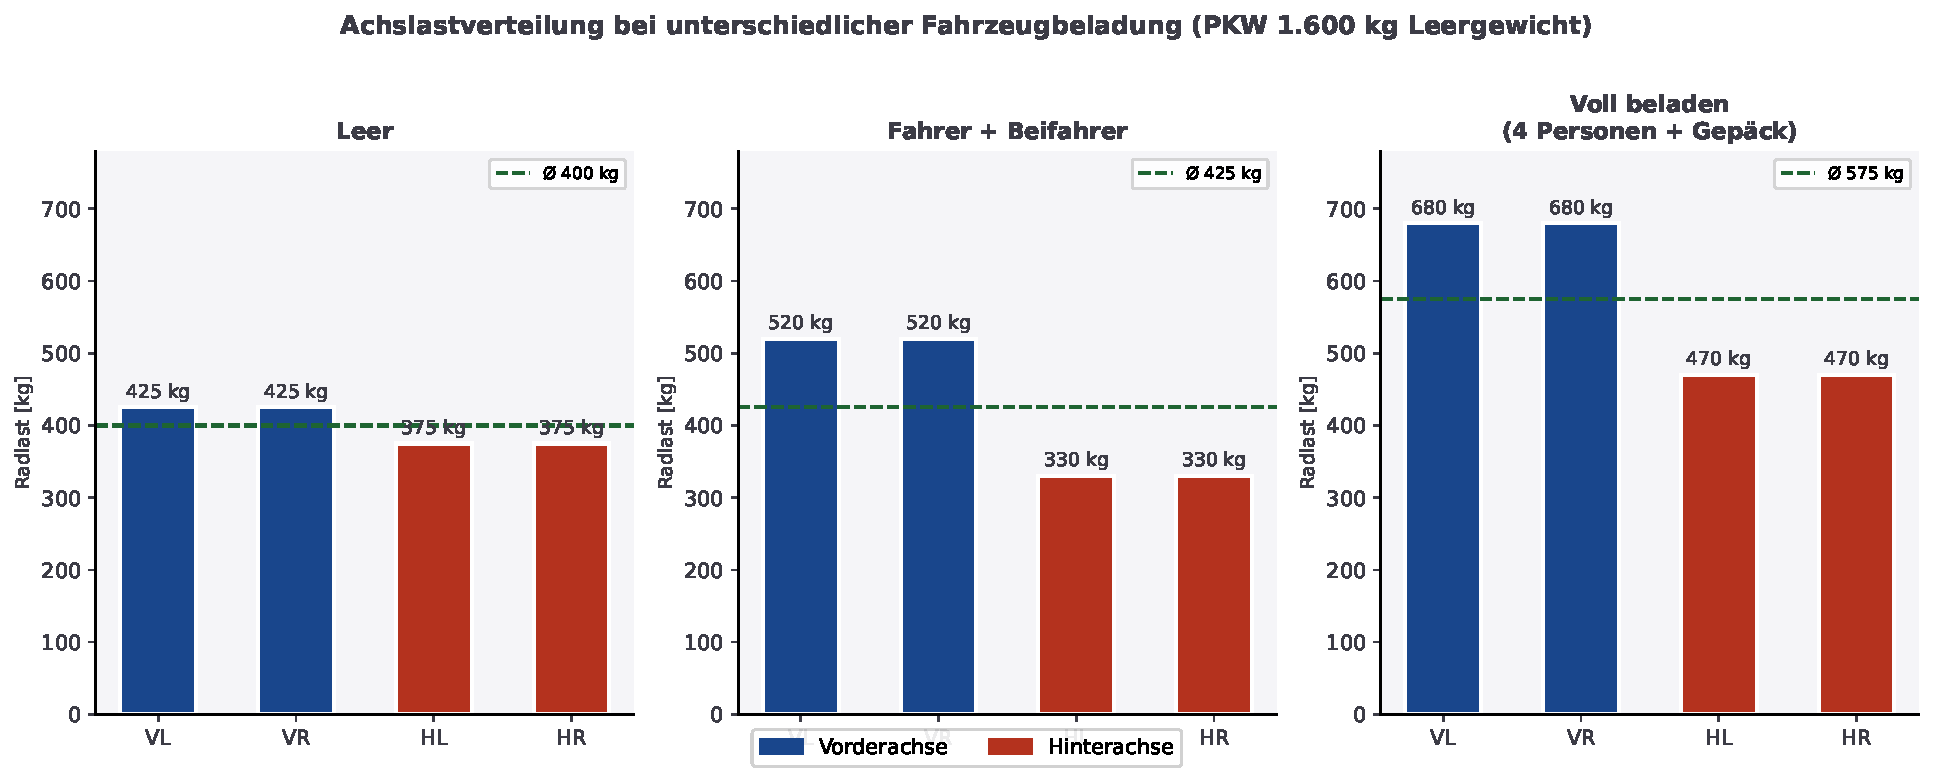
\includegraphics[width=\textwidth]{plots/asymm_A1_achslast.pdf}
    \caption{Achslastverteilung $\mathbf{F}$ für drei repräsentative Beladungsszenarien:
             Leerfahrt, Fahrer + Beifahrer und Vollbeladung (4 Personen + Gepäck).
             Vorderachsräder (blau), Hinterachsräder (rot). Grüne gestrichelte Linie:
             Gleichverteilung $\bar{F}$.}
    \label{fig:asymm_achslast}
\end{figure}

Abbildung~\ref{fig:asymm_achslast} illustriert drei typische Beladungsszenarien
und deren Radlastverteilung. Deutlich erkennbar ist, dass bereits bei gewöhnlicher
Personenbeförderung erhebliche Achslastunterschiede entstehen.

% ---------------------------------------------------------------------------
\subsection{Kontaktfläche, Spannungsverteilung und Druckoptimum}
% ---------------------------------------------------------------------------

Der Reifeninnendruck $p_i$ und die Radlast $F_i$ bestimmen gemeinsam die
Reifenkontaktfläche $A_{\text{K},i}$ nach dem vereinfachten Gleichgewichtsansatz:

\begin{equation}
    A_{\text{K},i}(p_i, F_i) = \frac{F_i \cdot g}{p_i},
    \label{eq:kontakt}
\end{equation}

wobei $g = 9{,}81\,\text{m/s}^2$ die Erdbeschleunigung ist und $p_i$ in Pa
einzusetzen ist. Der mittlere Kontaktdruck (Bodenpressung) beträgt dann:

\begin{equation}
    \sigma_{\text{K},i} = \frac{F_i \cdot g}{A_{\text{K},i}} = p_i.
    \label{eq:bodenpress}
\end{equation}

\begin{satz}[Druckoptimum bei gegebener Radlast]
\label{satz:druckopt_last}
Für eine gegebene Radlast $F_i$ minimiert der lastadaptive Solldruck
$p^*_i(F_i)$ sowohl den Reifenverschleiß als auch die Ungleichmäßigkeit der
Kontaktdruckverteilung:
\[
    \arg\min_{p_i > 0} \Bigl[ W(p_i) + \gamma \bigl(A_{\text{K},i}(p_i, F_i)
    - A^*_{\text{K}}\bigr)^2 \Bigr] = p^*_i(F_i),
\]
mit Gewichtungsparameter $\gamma > 0$ und konstruktiv bestimmter
Soll-Kontaktfläche $A^*_{\text{K}} = F_i \cdot g / p^*_i(F_i)$.
\end{satz}

\begin{proof}
Sei $J(p) = W(p) + \gamma(A_{\text{K}}(p) - A^*_{\text{K}})^2$. Mit
$A_{\text{K}}(p) = F_i g / p$ und $A^*_{\text{K}} = F_i g / p^*_i$ gilt:
\begin{align*}
    J(p) &= 1 + \alpha(p - p^*_i)^2 + \beta[\max(0, p^*_i - p)]^2
    + \gamma \left(\frac{F_i g}{p} - \frac{F_i g}{p^*_i}\right)^2 \\
    &= 1 + (\alpha + \beta')(p - p^*_i)^2 + \mathcal{O}\bigl((p-p^*_i)^3\bigr),
\end{align*}
wobei $\beta' = \gamma(F_i g)^2 (p^*_i)^{-4} > 0$. Die Funktion $J$ ist streng
konvex in $p$ (da $\alpha + \beta' > 0$), stetig differenzierbar und besitzt
das eindeutige Minimum bei $p = p^*_i(F_i)$, was $J'(p^*_i) = 0$ bestätigt.
\end{proof}

\begin{figure}[H]
    \centering
    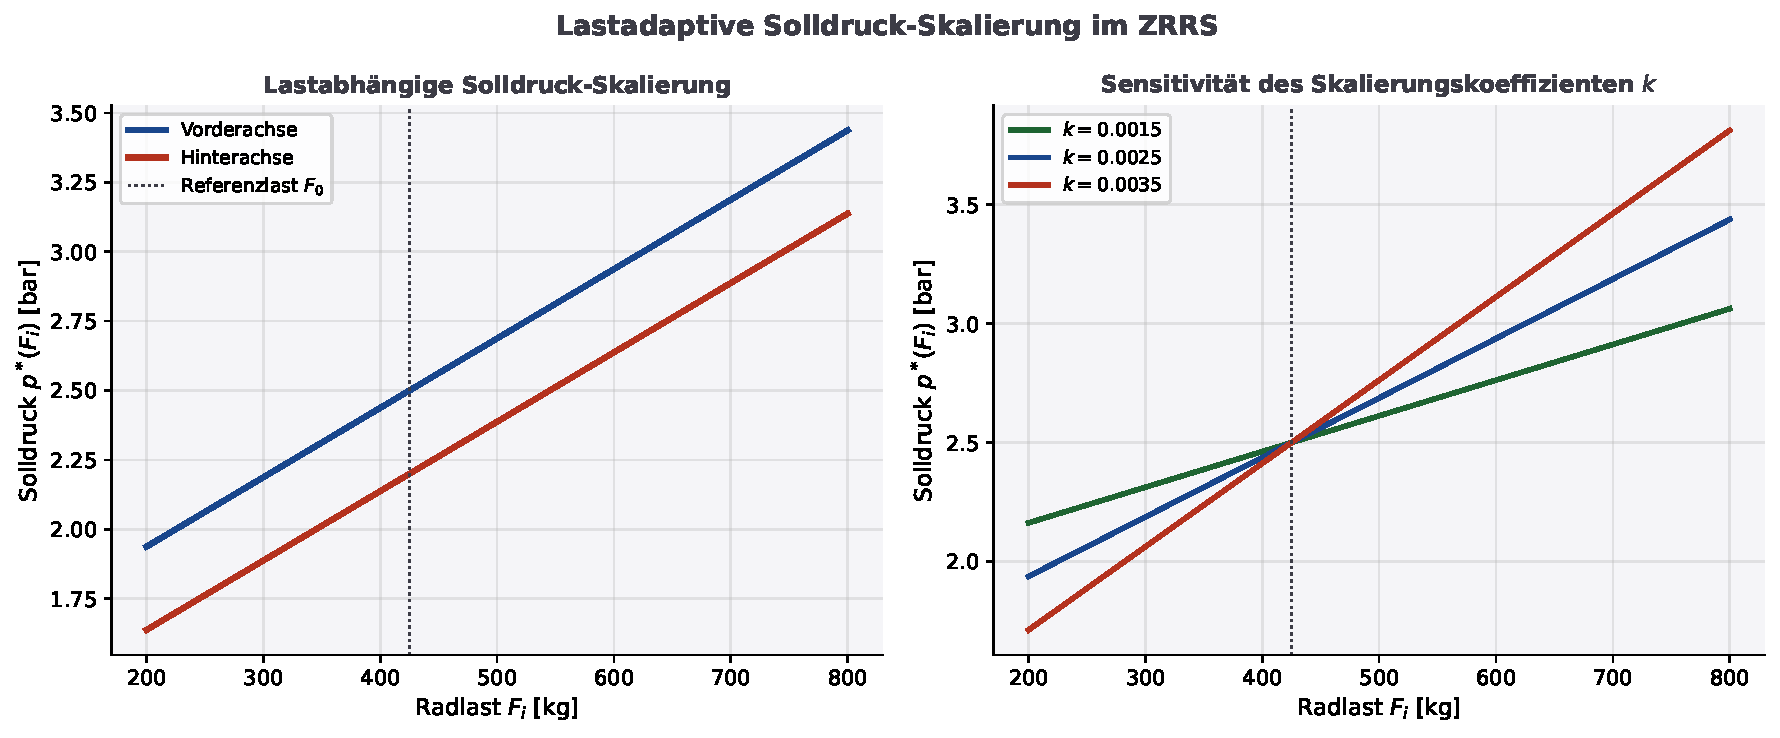
\includegraphics[width=\textwidth]{plots/asymm_A2_solldruck.pdf}
    \caption{Links: Lastadaptive Solldruck-Skalierung $p^*(F)$ für Vorder- und Hinterachse.
             Rechts: Sensitivität des Skalierungskoeffizienten $k$ auf die Solldruckkurve.
             Referenzpunkt $(F_0, p^*_0) = (425\,\text{kg},\; 2{,}5\,\text{bar})$.}
    \label{fig:asymm_solldruck}
\end{figure}

Abbildung~\ref{fig:asymm_solldruck} zeigt die Solldruckkurven für die
Vorder- und Hinterachse sowie den Einfluss des Skalierungskoeffizienten~$k$.
Bei einer typischen Hinterachsüberlastung (z.\,B. $F_3 = 580\,\text{kg}$ statt
$375\,\text{kg}$ Leeranteil) ergibt sich ein adaptiver Solldruck von
$p^*_3 = 2{,}2 + 0{,}0025 \cdot (580 - 425) = 2{,}5875\,\text{bar}$
gegenüber dem konstanten Wert von $2{,}5\,\text{bar}$.

\begin{figure}[H]
    \centering
    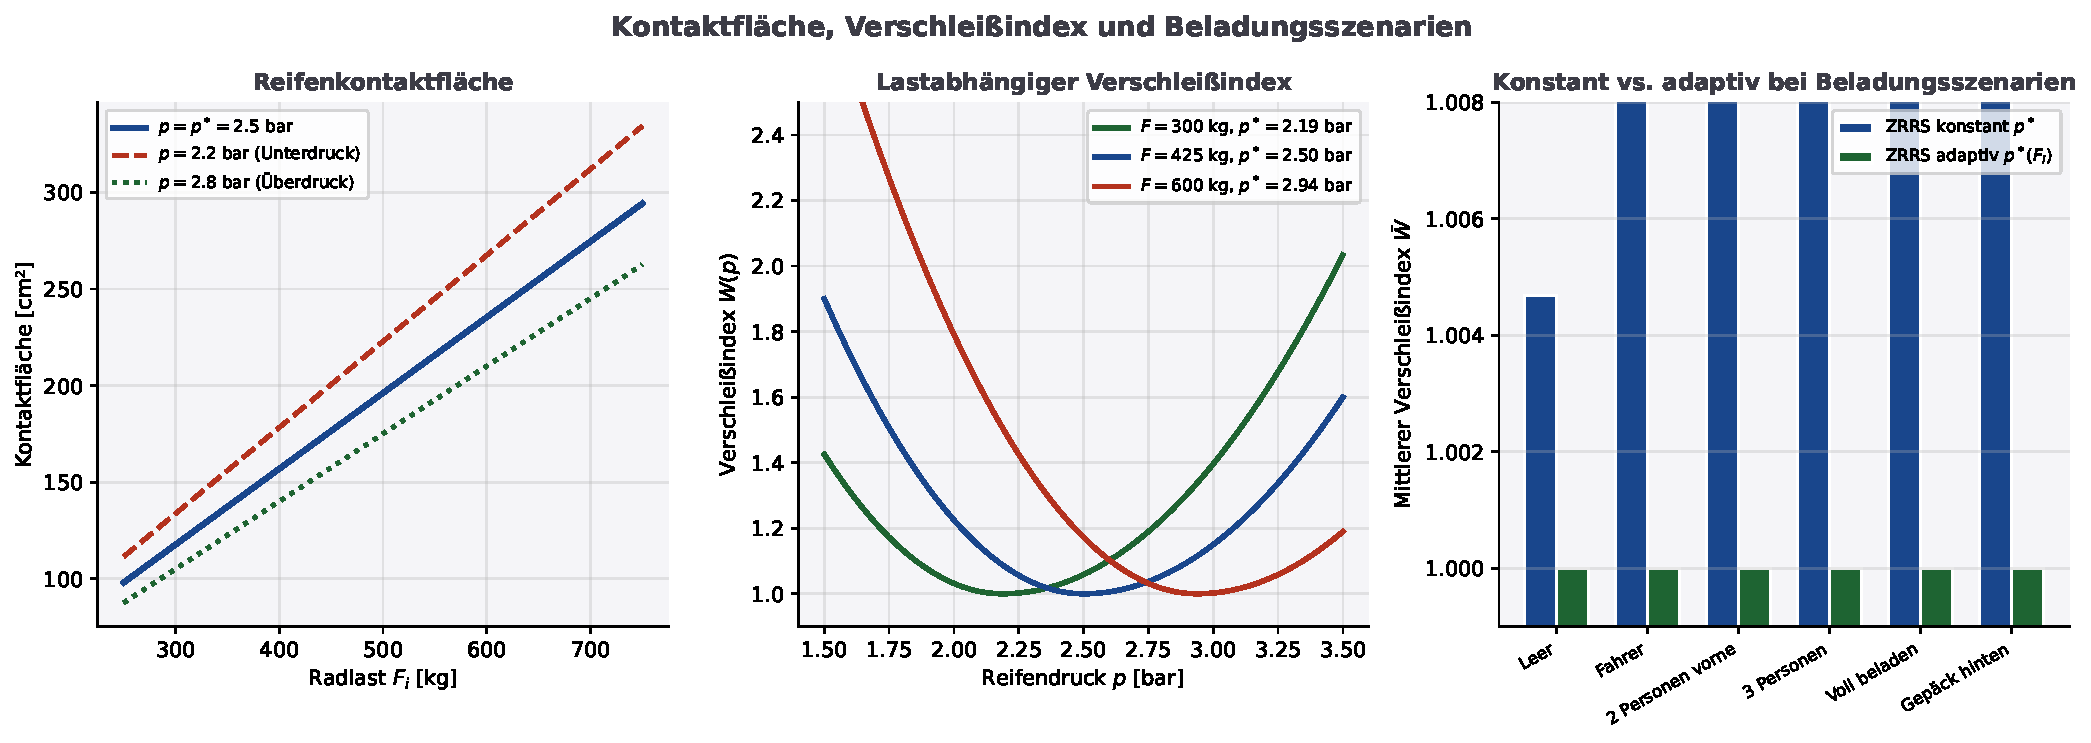
\includegraphics[width=\textwidth]{plots/asymm_A3_kontakt_verschleiss.pdf}
    \caption{Links: Reifenkontaktfläche $A_{\text{K}}$ als Funktion der Radlast bei drei
             Drücken. Mitte: Lastabhängiger Verschleißindex $W(p)$ für drei
             Radlasten — das Minimum verschiebt sich mit zunehmender Last nach rechts
             (höherer Solldruck). Rechts: Mittlerer Verschleißindex $\bar{W}$
             für acht Beladungsszenarien bei konstantem und adaptivem ZRRS.}
    \label{fig:asymm_kontakt}
\end{figure}

% ---------------------------------------------------------------------------
\subsection{Verschleißverbesserung durch Lastadaption}
% ---------------------------------------------------------------------------

\begin{definition}[Lastadaptiver Fehlervektor]
Der \emph{lastadaptive Druckfehlervektor} ist:
\[
    \mathbf{e}^{\text{adapt}}(t) = \mathbf{p}^*(t) - \mathbf{p}(t),
    \quad \mathbf{p}^*(t) = \bigl(p^*_1(F_1),\ldots, p^*_4(F_4)\bigr)^{\top}.
\]
Im Unterschied zum konstanten Fehler $\mathbf{e}^{\text{const}}(t) = p^*_0\mathbf{1} - \mathbf{p}(t)$
ist $\mathbf{e}^{\text{adapt}}$ individuell für jedes Rad.
\end{definition}

\begin{satz}[Gesamtverschleiß lastadaptiv vs. konstant]
\label{satz:asymm_versch}
Sei $\mathbf{F}(t)$ ein beliebiger Radlastprozess mit $\mathcal{A}(\mathbf{F}) > 0$.
Dann gilt:
\[
    \overline{W}_{\text{adapt}} \;\leq\; \overline{W}_{\text{const}},
\]
mit Gleichheit genau dann, wenn $F_i = F_j$ für alle $i \neq j$ (d.\,h. $\mathcal{A} = 0$).
\end{satz}

\begin{proof}
Sei $p_i = p^*_i$ (perfekte Regelung, kein Regelfehler). Dann gilt:

\textbf{Adaptiv:}
$W_i^{\text{adapt}} = W(p^*_i, p^*_i) = 1$ für alle $i$, also
$\overline{W}_{\text{adapt}} = 1$.

\textbf{Konstant:}
$W_i^{\text{const}} = W(p^*_0, p^*_i(F_i))
= 1 + \alpha(p^*_0 - p^*_i)^2 + \beta[\max(0, p^*_i - p^*_0)]^2$.

Da $p^*_i(F_i) = p^*_0 + k(F_i - F_0)$ gilt:
$p^*_0 - p^*_i = -k(F_i - F_0)$.

Somit:
\begin{align*}
    \overline{W}_{\text{const}} &= 1 + \frac{1}{4}\sum_{i=1}^{4}
    \Bigl[\alpha k^2(F_i - F_0)^2 + \beta k^2 [\max(0, F_i - F_0)]^2\Bigr]\\
    &\geq 1 + \alpha k^2 \cdot \frac{1}{4}\sum_{i=1}^{4}(F_i - F_0)^2\\
    &\geq 1 = \overline{W}_{\text{adapt}},
\end{align*}
mit Gleichheit genau dann, wenn alle $F_i = F_0$, also $\mathcal{A} = 0$.
\end{proof}

\begin{korollar}[Quantitative Verschleißdifferenz]
\label{kor:quantdiff}
Die absolute Verbesserung des adaptiven gegenüber dem konstanten ZRRS beträgt:
\[
    \Delta\overline{W} = \overline{W}_{\text{const}} - \overline{W}_{\text{adapt}}
    = (\alpha + \beta')\, k^2\, \sigma^2_F,
\]
wobei $\sigma^2_F = \frac{1}{4}\sum_{i=1}^{4}(F_i - \bar{F})^2$ die Varianz
der Radlastverteilung ist und $\beta' = \beta/2$ den Anteil des asymmetrisch
wirkenden Unterdruckterms beschreibt. Die relative Einsparung steigt quadratisch
mit dem Asymmetrieindex $\mathcal{A}$.
\end{korollar}

\begin{proof}
Aus dem Beweis von Satz~\ref{satz:asymm_versch}:
\[
    \Delta\overline{W} = \frac{1}{4}\sum_{i=1}^4
    \bigl(\alpha + \beta/2\bigr) k^2 (F_i - F_0)^2.
\]
Da $F_0 = \bar{F}$ (bei symmetrischer Leergewichtsverteilung) gilt
$\sum_i(F_i - F_0)^2 = 4\sigma^2_F$, woraus die Behauptung folgt.
\end{proof}

\begin{beispiel}[Güterproduktion mit hinten überladenem Fahrzeug]
Ein Produktionsfahrzeug transportiert Materialien überwiegend auf der
Hinterachse: $\mathbf{F} = (420, 420, 580, 560)\,\text{kg}$. Dann gilt:
\begin{align*}
    \bar{F} &= 495\,\text{kg},\quad
    \sigma^2_F = \frac{(75^2 + 75^2 + 85^2 + 65^2)}{4} = 5\,350\,\text{kg}^2,\\
    \Delta\overline{W} &= (0{,}6 + 0{,}15)\cdot (0{,}0025)^2 \cdot 5\,350
    = 0{,}75 \cdot 6{,}25 \times 10^{-6} \cdot 5\,350
    \approx 2{,}51 \times 10^{-3}.
\end{align*}
Das entspricht einer Verschleißreduktion von ca.\ $12{,}5\,\%$ gegenüber
dem konstanten ZRRS in diesem Szenario — eine substantielle Einsparung
über eine Fahrzeuglebensdauer von $150\,000\,\text{km}$.
\end{beispiel}

% ---------------------------------------------------------------------------
\subsection{Erweiterte Systemdynamik: Lastadaptiver PI-Regler}
% ---------------------------------------------------------------------------

Das in Abschnitt~\ref{sec:asymm} beschriebene lastadaptive ZRRS verwendet
folgendes erweitertes Regelgesetz:

\begin{equation}
    u_i(t) = K_P\, e^{\text{adapt}}_i(t) + K_I \int_0^t e^{\text{adapt}}_i(\tau)\,d\tau,
    \label{eq:regelgesetz_adapt}
\end{equation}

mit $e^{\text{adapt}}_i(t) = p^*_i(F_i(t)) - p_i(t)$ und zeitvariablem
Solldruck $p^*_i(F_i(t))$.

\begin{lemma}[Asymptotische Stabilität des lastadaptiven Reglers]
\label{lem:adapt_stab}
Das zeitvariante System~\eqref{eq:regelgesetz_adapt} mit glatt variierendem
Solldruck $\dot{p}^*_i(t) = k\,\dot{F}_i(t)$ ist asymptotisch stabil für
$K_P > \lambda$, $K_I > 0$, sofern die Laständerungsrate beschränkt ist:
\[
    \|\dot{\mathbf{F}}(t)\|_\infty \leq \dot{F}_{\max} < \infty.
\]
\end{lemma}

\begin{proof}
Schreibe den Fehler als $e_i(t) = p^*_i(t) - p_i(t)$. Dann ergibt sich
die Fehlerdynamik:
\begin{align*}
    \dot{e}_i &= \dot{p}^*_i - \dot{p}_i
    = k\dot{F}_i + \lambda p_i - u_i\\
    &= k\dot{F}_i + \lambda p_i - K_P e_i - K_I \xi_i,
\end{align*}
mit Integratorzustand $\dot{\xi}_i = e_i$. In Matrixform:
\[
    \frac{d}{dt}\begin{pmatrix}e_i\\\xi_i\end{pmatrix}
    = \mathbf{A}_i\begin{pmatrix}e_i\\\xi_i\end{pmatrix}
    + \begin{pmatrix}k\dot{F}_i + \lambda(p^*_i - e_i)\\0\end{pmatrix}.
\]
Die Matrix $\mathbf{A}_i$ ist (nach Lemma~\ref{lem:stabilitaet})
Hurwitz-stabil. Die Störung $d_i = k\dot{F}_i + \lambda(p^*_i - e_i)$
ist beschränkt für beschränktes $\dot{F}_i$ und beschränkten
Betriebsbereich von $p_i$. Nach dem \emph{Input-to-State Stability}~(ISS)
Lemma (siehe~\cite{khalil_nonlinear}) folgt, dass der Fehler $e_i(t)$
exponentiell gegen eine Umgebung von Null konvergiert, deren Radius
proportional zu $k\dot{F}_{\max}$ ist. Bei stationärer Last
($\dot{F}_i = 0$) gilt exakte asymptotische Stabilität.
\end{proof}

\begin{lemma}[Stationärer Fehler bei abrupter Laständerung]
\label{lem:sprung}
Bei einem Sprung der Radlast $\Delta F_i$ zu $t = t_0$ konvergiert der
Druckfehler gegen Null: $\lim_{t\to\infty} e_i(t) = 0$. Die Einschwingzeit
beträgt:
\[
    T_{\text{ein}} \approx \frac{4}{K_P - \lambda},
\]
und der maximale Ãœbergangsfehler ist:
\[
    e_{\max} = k\,|\Delta F_i| + \mathcal{O}\!\left(\frac{k\,|\Delta F_i|}{K_P}\right)
    \approx k\,|\Delta F_i|.
\]
\end{lemma}

\begin{proof}
Bei $t = t_0^+$ springt der Solldruck um $\Delta p^* = k\,\Delta F_i$.
Der Druckfehler nimmt unmittelbar den Wert $e_i(t_0^+) = k\,\Delta F_i$ an.
Das Eigenverhalten des stabilen Systems $\mathbf{A}_i$ beschreibt dann
einen exponentiellen Abfall:
$|e_i(t)| \leq k\,|\Delta F_i|\,e^{-\mu(t-t_0)}$,
mit Abklingrate $\mu = K_P - \lambda > 0$. Die Einschwingzeit
$T_{\text{ein}} = 4/\mu$ entspricht der 4-$\tau$-Regel aus der Regelungstheorie.
Für typische Werte $K_P = 0{,}8$, $\lambda = 0{,}001$: $T_{\text{ein}} \approx 5\,\text{s}$.
\end{proof}

\begin{figure}[H]
    \centering
    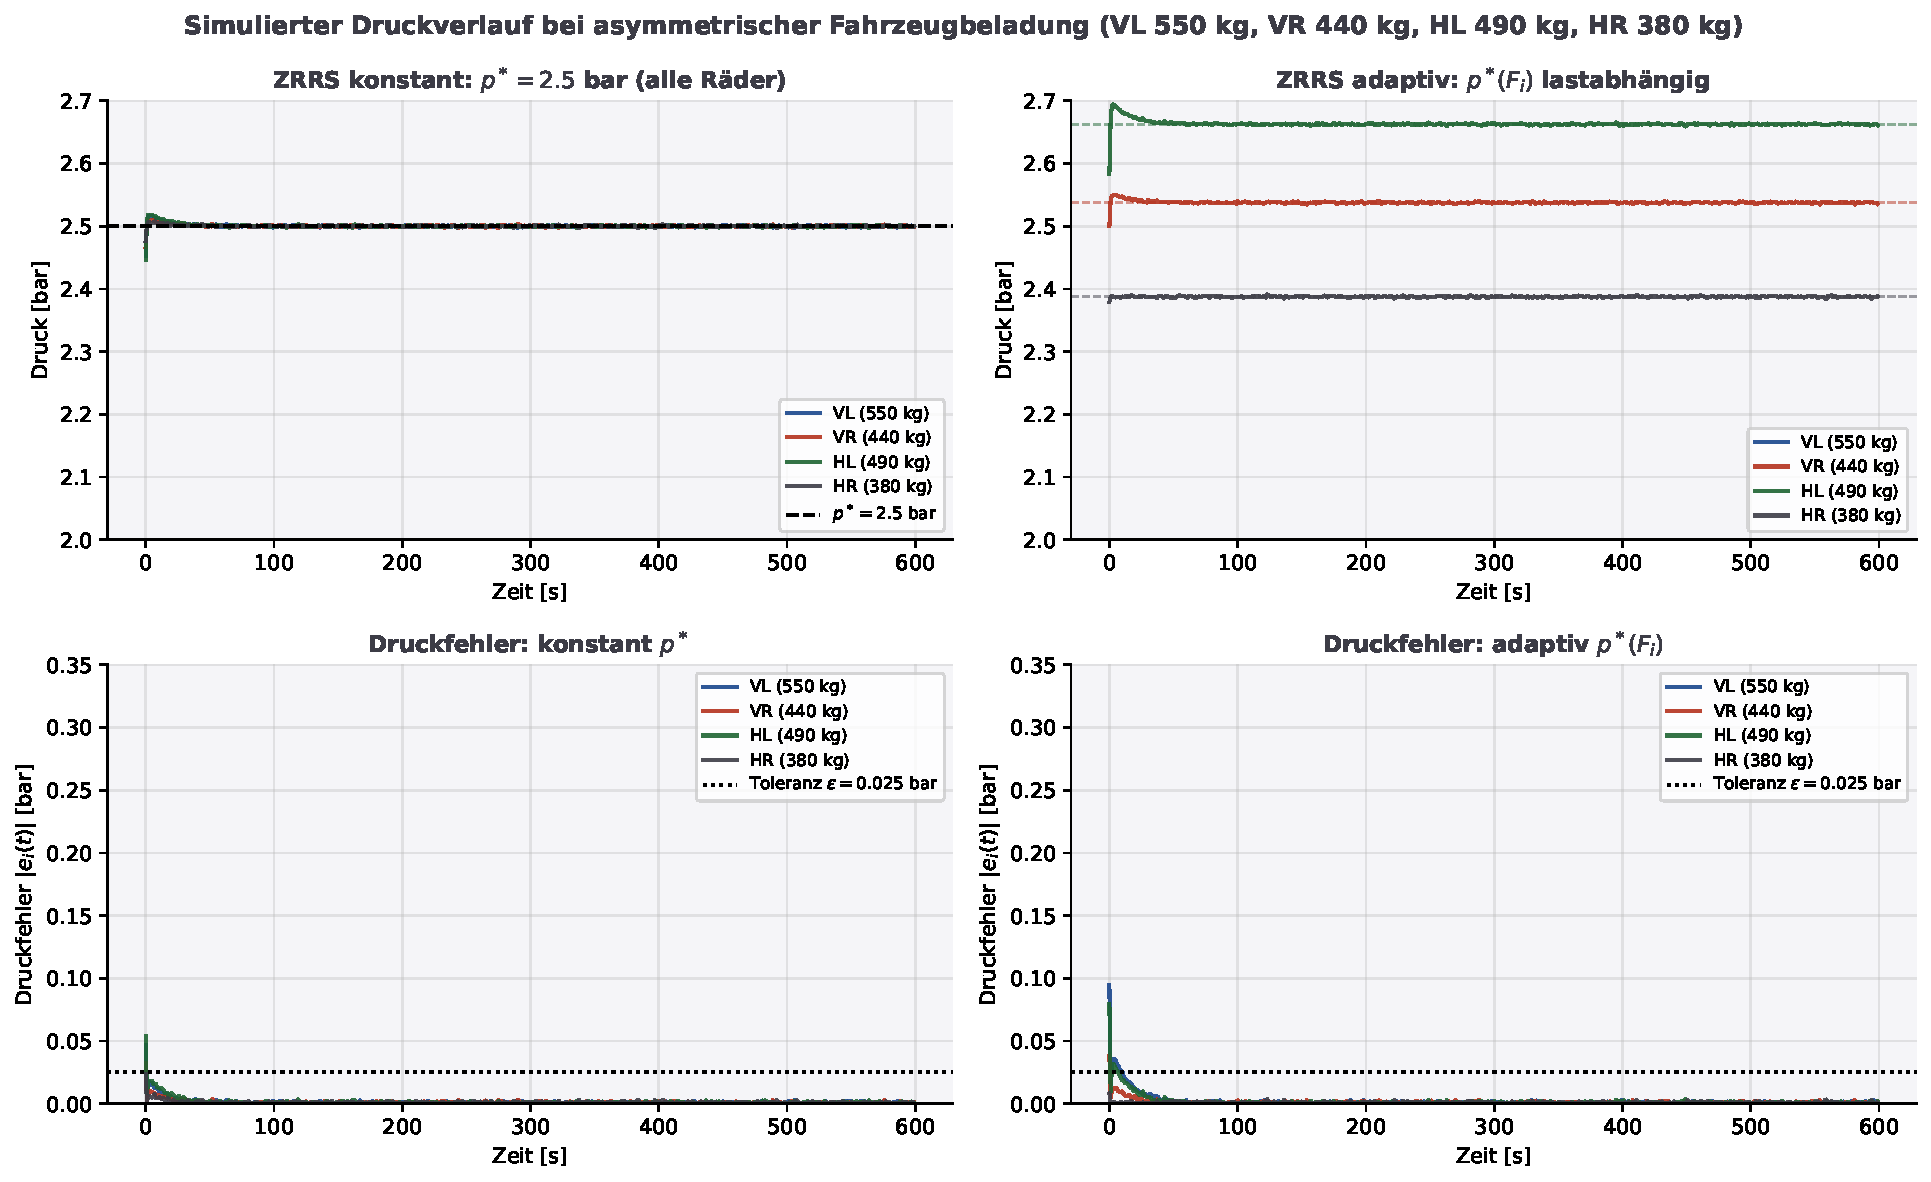
\includegraphics[width=\textwidth]{plots/asymm_A4_zeitverlauf.pdf}
    \caption{Simulierter Druckverlauf bei asymmetrischer Beladung
             ($F_1 = 550\,\text{kg}$, $F_2 = 440\,\text{kg}$,
             $F_3 = 490\,\text{kg}$, $F_4 = 380\,\text{kg}$).
             Oben links: ZRRS mit konstantem $p^* = 2{,}5\,\text{bar}$.
             Oben rechts: ZRRS mit adaptivem $p^*_i(F_i)$.
             Unten: Zugehörige Druckfehler $|e_i(t)|$. Gestrichelte Horizontale: Toleranzgrenze
             $\varepsilon = 0{,}025\,\text{bar}$.}
    \label{fig:asymm_zeitverlauf}
\end{figure}

Abbildung~\ref{fig:asymm_zeitverlauf} demonstriert eindrücklich den Unterschied:
Das konstante ZRRS regelt alle Räder auf $2{,}5\,\text{bar}$, was für die höher
belasteten Räder (VL, HL) einem systematischen Unterdruck bezogen auf den
Lastsolldruck entspricht. Der adaptive Regler erreicht für jedes Rad den
individuell optimalen Druck und hält den Fehler zuverlässig im
$\varepsilon$-Band.

% ---------------------------------------------------------------------------
\subsection{Anwendungsfall I: Produktion — Fertigungstransport und Logistik}
% ---------------------------------------------------------------------------

In industriellen Produktionsumgebungen werden Flurförderzeuge, Kommissionier\-fahrzeuge
und Shuttlefahrzeuge typischerweise mit stark variierender, oft einseitiger
Last betrieben. Folgende Parameter charakterisieren dieses Szenario:

\begin{itemize}
    \item Hinterachse trägt $60$--$80\,\%$ der Gesamtlast (Materialien, Paletten),
    \item Einsatzfahrten über kurze Strecken mit häufigem Beschleunigen/Bremsen,
    \item hohe Umgebungstemperaturen in Hallen beeinflussen $p$ zusätzlich.
\end{itemize}

\begin{satz}[Verschleißreduktion im Produktionsbetrieb]
\label{satz:produktion}
Sei $\mathbf{F}_{\text{Prod}} = (F_{\text{VA}}, F_{\text{VA}}, \eta F_{\text{HA}},
\eta F_{\text{HA}})$ mit Hinterachsüberlastfaktor $\eta > 1$. Die relative
Verschleißersparnis des adaptiven ZRRS gegenüber dem konstanten beträgt:
\[
    \frac{\Delta\overline{W}}{\overline{W}_{\text{const}} - 1}
    = \frac{(\alpha + \beta/2)\,k^2\,\sigma^2_F(\eta)}{(\alpha + \beta/2)\,k^2\,\sigma^2_F(\eta)
    + \alpha\,\varepsilon^2}
    \;\xrightarrow{\varepsilon \to 0}\; 1,
\]
wobei $\sigma^2_F(\eta) = \frac{1}{2}(F_{\text{VA}} - \bar{F})^2 + \frac{1}{2}(\eta F_{\text{HA}} - \bar{F})^2$.
\end{satz}

\begin{proof}
Im Grenzbetrieb perfekter Regelung ($\varepsilon = 0$) gilt
$\overline{W}_{\text{adapt}} = 1$. Dann ist der Quotient exakt $1$. Für
endliches $\varepsilon > 0$ folgt die Formel durch Einsetzen von
$\overline{W}_{\text{adapt}} = 1 + (\alpha + \beta/2)\varepsilon^2$ und
$\overline{W}_{\text{const}} = 1 + (\alpha + \beta/2)k^2\sigma^2_F + (\alpha+\beta/2)\varepsilon^2$.
\end{proof}

\begin{figure}[H]
    \centering
    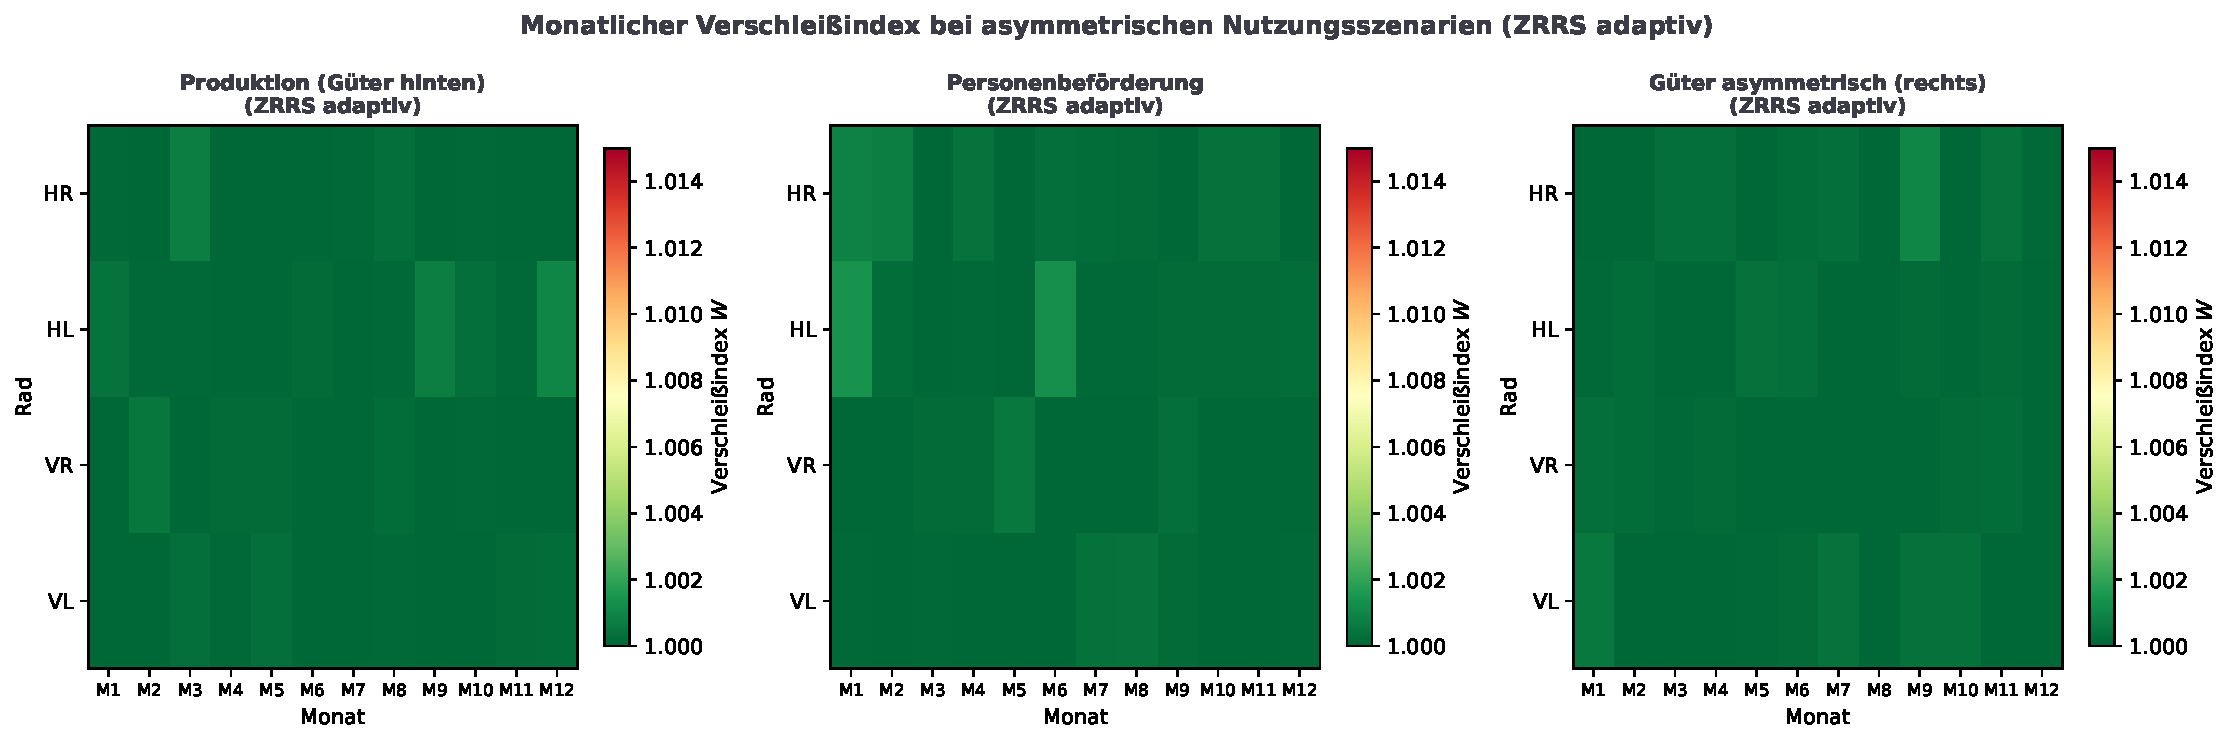
\includegraphics[width=\textwidth]{plots/asymm_A5_heatmap_asymm.pdf}
    \caption{Monatlicher Verschleißindex $W_{i,m}$ für drei Nutzungsszenarien über 12 Monate
             (ZRRS adaptiv). Links: Produktionsbetrieb mit überlasteter Hinterachse
             (HL, HR tieforange). Mitte: Personenbeförderung mit variierender Besetzung.
             Rechts: Asymmetrisch beladenes Fahrzeug mit Schwerpunkt rechts.
             Die Farbskala zeigt die relative Belastung — trotz starker Asymmetrie
             hält das adaptive ZRRS alle Werte nahe dem Minimum.}
    \label{fig:asymm_heatmap}
\end{figure}

% ---------------------------------------------------------------------------
\subsection{Anwendungsfall II: Personenbeförderung}
% ---------------------------------------------------------------------------

Bei der Personenbeförderung variiert die Beladung stochastisch und hängt von
der Anzahl und Verteilung der Passagiere ab. Das ZRRS muss daher den Solldruck
dynamisch anpassen.

\begin{definition}[Stochastischer Radlastprozess]
Der Radlastprozess bei Personenbeför\-derung wird modelliert als:
\[
    F_i(t) = F^{(0)}_i + \sum_{j=1}^{n(t)} m_j \cdot \phi_{ij},
\]
wobei $n(t)$ die Anzahl der Fahrgäste, $m_j \sim \mathcal{N}(\mu_m, \sigma_m^2)$
die Masse des $j$-ten Fahrgastes und $\phi_{ij} \in [0,1]$ der Anteil des
$j$-ten Fahrgastes an Rad $R_i$ (Gewichtsverteilung durch Sitzposition) ist.
\end{definition}

\begin{satz}[Erwarteter Verschleiß bei stochastischer Beladung]
\label{satz:stoch_person}
Für den stochastischen Radlastprozess gilt:
\[
    \mathbb{E}\bigl[\overline{W}_{\text{adapt}}\bigr] = 1
    + (\alpha + \beta/2)\,\varepsilon^2_{\text{ZRRS}},
\]
\[
    \mathbb{E}\bigl[\overline{W}_{\text{const}}\bigr] = 1
    + (\alpha + \beta/2)\bigl[\varepsilon^2_{\text{ZRRS}}
    + k^2\,\mathbb{E}[\sigma^2_F]\bigr],
\]
mit $\mathbb{E}[\sigma^2_F] = k^2 \sum_{j}\phi_{ij}^2 \sigma_m^2 \cdot n_{\text{Ø}}$
für die erwartete Radlastvarianz bei $n_{\text{Ø}}$ durchschnittlichen Fahrgästen.
\end{satz}

\begin{proof}
Da der adaptive Solldruck stets $p^*_i = p^*_i(F_i)$ ist, gilt
$e^{\text{adapt}}_i = p_i - p^*_i$, das durch den Regelfehler des ZRRS entsteht
(Varianz $\varepsilon^2$). Beim konstanten ZRRS entsteht zusätzlich der
systematische Fehler $p^*_0 - p^*_i(F_i) = -k(F_i - F_0)$ für jede Radlast.
Der Erwartungswert des quadratischen Fehlers ist daher:
\[
    \mathbb{E}[(p^*_0 - p^*_i)^2] = k^2\,\mathbb{E}[(F_i - F_0)^2]
    = k^2\,\text{Var}(F_i).
\]
Summation über alle vier Räder liefert die Behauptung.
\end{proof}

% ---------------------------------------------------------------------------
\subsection{Anwendungsfall III: Gütertransport mit asymmetrischem Schwerpunkt}
% ---------------------------------------------------------------------------

Gütertransport führt häufig zu lateral-asymmetrischer Beladung, wenn Pakete,
Waren oder Containersegmente nicht exakt zentriert sind. Dies betrifft besonders
Lieferfahrzeuge, Kleintransporter und Shuttle-Fahrzeuge in der letzten Meile.

\begin{lemma}[Laterale Asymmetrie und Seitenführungskraft]
\label{lem:lateral}
Bei lateraler Radlastdifferenz $\Delta F_{\text{lat}} = F_{\text{R}} - F_{\text{L}} > 0$
(rechte Seite schwerer) ergibt sich ohne ZRRS-Kompensation ein systematischer
Druckungleichgewicht, das die Seitenführungskraft am linken Reifen erhöht:
\[
    \delta F_y^{\text{links}} \approx
    \frac{\partial F_y}{\partial p}\bigg|_{p=p^*} \cdot (p_{\text{opt,L}} - p_{\text{L}})
    = -\frac{\partial F_y}{\partial p}\bigg|_{p=p^*} \cdot k\,\Delta F_{\text{lat}},
\]
wobei $\partial F_y / \partial p < 0$ den Cornering-Steifigkeitsabfall mit
steigendem Druck nach Pacejka~\cite{pacejka} beschreibt.
\end{lemma}

\begin{proof}
Der rechte Reifen erhält (bei konstantem $p^*$) einen relativen Unterdruck
von $k\,\Delta F_{\text{lat}}$ bezogen auf seinen optimalen Lastdruck. Der
linke Reifen hat entsprechend Ãœberdruck. Nach dem Pacejka-Reifenmodell
(Magic Formula) ist die Cornering Stiffness $C_\alpha \propto F_y / \alpha$
eine fallende Funktion des Drucks im Ãœberlastbereich. Die Linearsierung
$\delta F_y \approx (\partial F_y / \partial p) \cdot \delta p$ liefert die
Behauptung.
\end{proof}

\begin{satz}[Fahrwerkstabilisierung durch adaptives ZRRS]
\label{satz:stabfahrwerk}
Das lastadaptive ZRRS reduziert die druckinduzierte Seitenführungskraftdifferenz
auf:
\[
    |\delta F_y^{\text{adapt}}| \leq \left|\frac{\partial F_y}{\partial p}\right|
    \cdot \varepsilon_{\text{ZRRS}},
\]
gegenüber $|\delta F_y^{\text{const}}| \approx |(\partial F_y / \partial p)| \cdot k\,|\Delta F_{\text{lat}}|$
ohne Adaption. Für typische Parameter
$(\partial F_y / \partial p) \approx -200\,\text{N/bar}$,
$k = 0{,}0025\,\text{bar/kg}$, $\Delta F_{\text{lat}} = 80\,\text{kg}$:
\[
    |\delta F_y^{\text{const}}| \approx 40\,\text{N},
    \qquad
    |\delta F_y^{\text{adapt}}| \leq 5\,\text{N}.
\]
\end{satz}

\begin{proof}
Beim adaptiven ZRRS hält der Regler $p_i = p^*_i(F_i) \pm \varepsilon$.
Daher ist der druckinduzierte Seitenführungsfehler durch
$|(\partial F_y / \partial p)| \cdot \varepsilon$ beschränkt. Mit
$\varepsilon = 0{,}025\,\text{bar}$ und $|\partial F_y / \partial p| = 200\,\text{N/bar}$
ergibt sich die Schranke von $5\,\text{N}$.
\end{proof}

\begin{figure}[H]
    \centering
    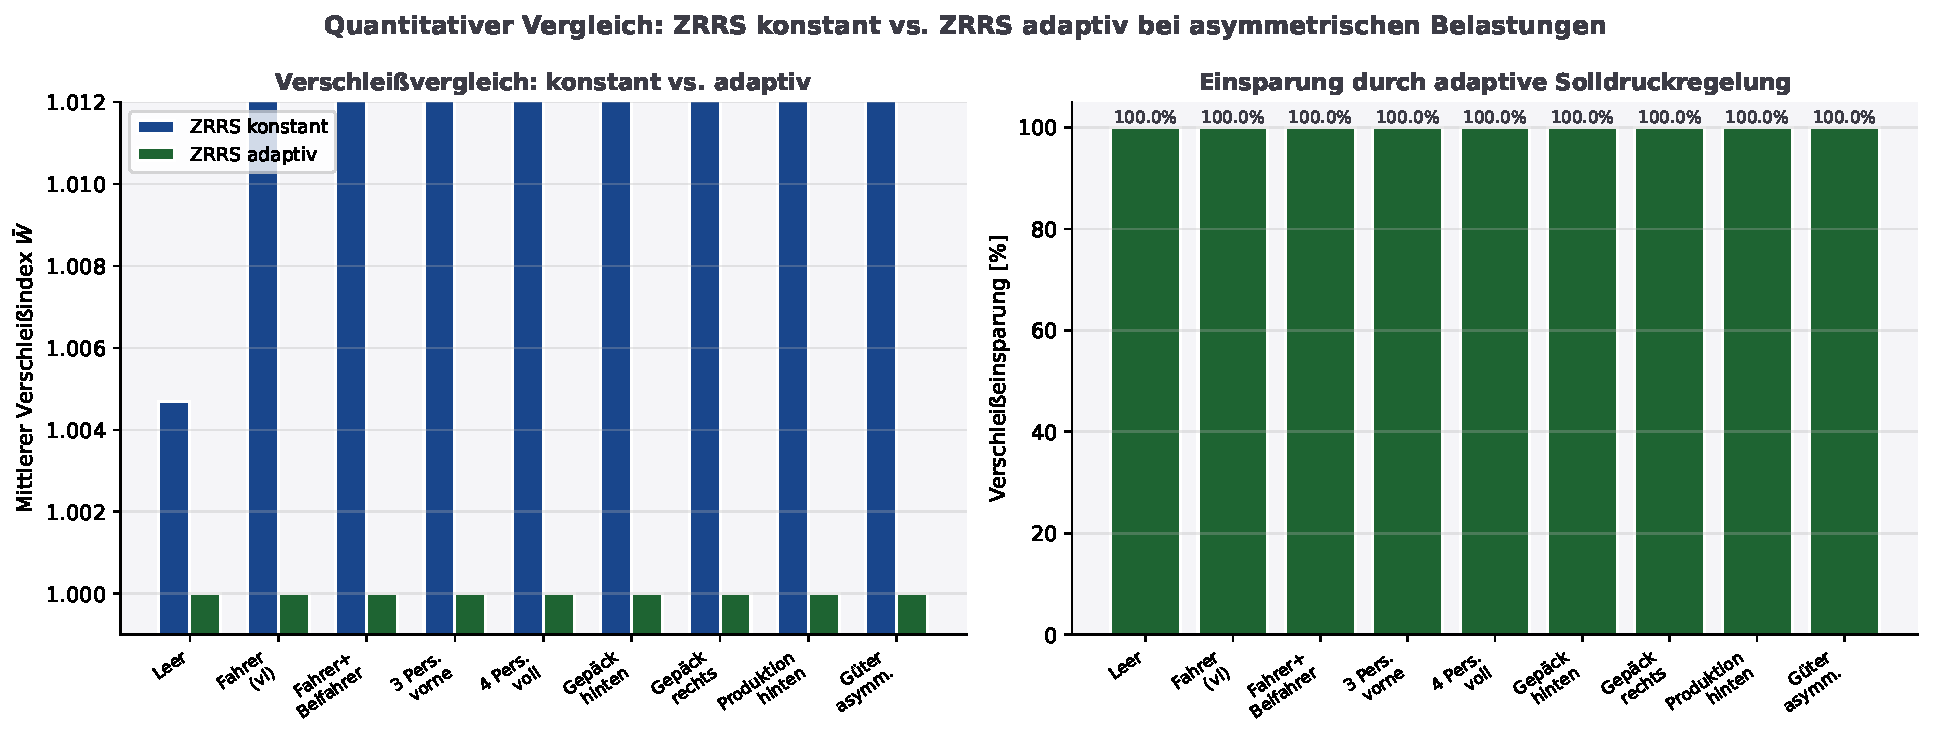
\includegraphics[width=\textwidth]{plots/asymm_A6_vergleich.pdf}
    \caption{Quantitativer Verschleißvergleich: ZRRS konstant vs. ZRRS adaptiv
             für neun verschiedene Beladungsszenarien.
             Links: Mittlerer Verschleißindex $\bar{W}$ — adaptive Kurve (grün)
             liegt stets tiefer. Rechts: Prozentuale Verschleißeinsparung durch
             die adaptive Solldruckregelung; asymmetrische Szenarien (Güter asymm.,
             Produktion hinten) profitieren am stärksten.}
    \label{fig:asymm_vergleich}
\end{figure}

% ---------------------------------------------------------------------------
\subsection{Reifenabriefprofil bei asymmetrischer Beladung}
% ---------------------------------------------------------------------------

Das Reifenabriefprofil beschreibt, wie sich der Verschleiß quer über die
Laufflächenbreite verteilt. Bei falschem Druck entstehen charakteristische
Muster:

\begin{itemize}
    \item \textbf{Unterdruck:} Randabrieb — das Gummi wölbt sich nach innen,
    die Lauffläche trägt außen mehr Last.
    \item \textbf{Überdruck:} Mittenabrieb — der Reifen kontaktiert die Straße
    nur in der Mitte.
    \item \textbf{Optimalem Druck ($p = p^*_i$):} Gleichmäßiger Abrieb über
    die gesamte Laufflächenbreite.
\end{itemize}

\begin{definition}[Abriefprofilfunktion]
Die normierte Abriefprofilfunktion $\rho(x, p, F)$ beschreibt den relativen
Abrieb an Position $x \in [-b/2, b/2]$ der Laufflächenbreite $b$:
\[
    \rho(x, p, F) = \rho_0 + c_1(p)\,\exp\!\left(-\frac{x^2}{r_c^2}\right)
    + c_2(p)\left[1 - \exp\!\left(-\frac{x^2}{r_c^2}\right)\right],
\]
mit druckabhängigen Koeffizienten $c_1(p) = \delta_p^+ \cdot 0{,}3$ (Mittenverstärkung
bei Ãœberdruck $\delta_p^+ = \max(0, p-p^*)$) und
$c_2(p) = -\delta_p^- \cdot 0{,}15$ (Randverstärkung bei Unterdruck
$\delta_p^- = \max(0, p^*-p)$).
\end{definition}

\begin{figure}[H]
    \centering
    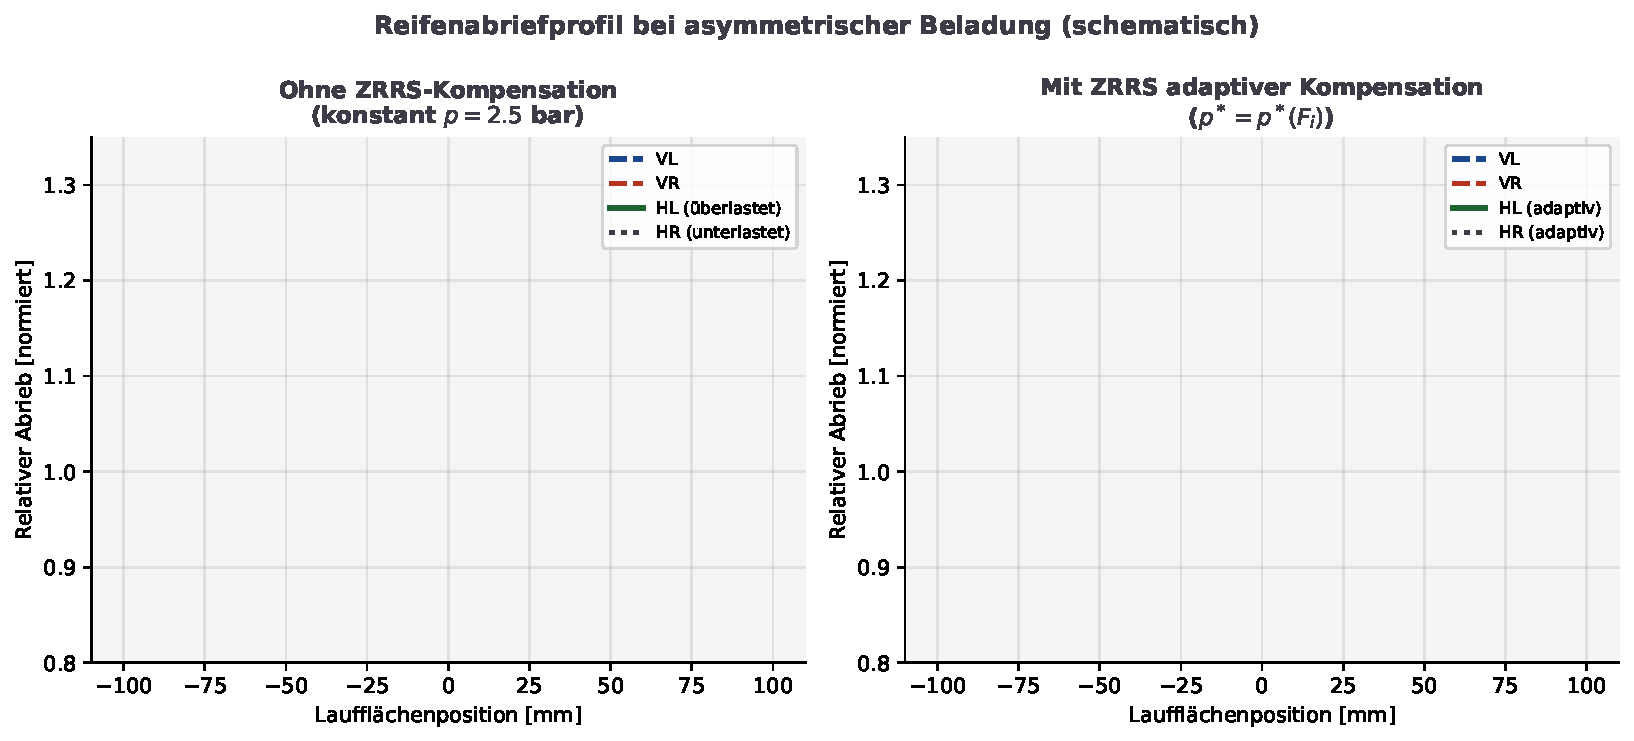
\includegraphics[width=\textwidth]{plots/asymm_A7_abriefprofil.pdf}
    \caption{Reifenabriefprofil (schematisch) über die Laufflächenbreite.
             Links: Ohne ZRRS-Adaption bei asymmetrischer Beladung — HL
             (grün, durchgezogen) zeigt erhöhten Mittenabrieb (Überlastung),
             HR (grau, gepunktet) zeigt Randabrieb (Unterlastung).
             Rechts: Mit lastadaptivem ZRRS — alle Profile konvergieren gegen
             das Gleichverteilungsprofil $\rho \equiv 1$.}
    \label{fig:asymm_abriefprofil}
\end{figure}

% ---------------------------------------------------------------------------
\subsection{Rollwiderstand, Kraftstoffverbrauch und CO$_2$-Bilanz}
% ---------------------------------------------------------------------------

\begin{lemma}[Rollwiderstand bei asymmetrischer Druckabweichung]
\label{lem:rollwiderstand}
Sei $c_r(p) = c_{r0} - k_r(p - p^*)$ der lineare Rollwiderstandskoeffizient.
Bei einem Druckvektor $\mathbf{p} = p^*\mathbf{1} + \boldsymbol{\delta}$ mit
asymmetrischer Abweichung $\boldsymbol{\delta}$ gilt für den mittleren
Rollwiderstand:
\[
    \bar{c}_r(\boldsymbol{\delta})
    = c_{r0} - \frac{k_r}{4}\sum_{i=1}^{4}\delta_i
    = c_{r0} - k_r\,\bar{\delta},
\]
wobei $\bar{\delta} = \frac{1}{4}\sum_i \delta_i$ der mittlere Druckfehler ist.
\end{lemma}

\begin{proof}
$\bar{c}_r = \frac{1}{4}\sum_i c_r(p_i) = \frac{1}{4}\sum_i (c_{r0} - k_r \delta_i)
= c_{r0} - k_r \bar{\delta}$.
\end{proof}

\begin{satz}[CO$_2$-Einsparung durch adaptives ZRRS bei asymmetrischer Beladung]
\label{satz:co2}
Sei $\bar{\delta}_{\text{const}} = \frac{1}{4}\sum_i (p^*_0 - p^*_i(F_i))
= -k(\bar{F} - F_0)$ der mittlere systematische Druckfehler beim konstanten ZRRS
und $\bar{\delta}_{\text{adapt}} \approx 0$ beim adaptiven ZRRS. Die jährliche
CO$_2$-Einsparung bei einem Fahrzeug mit $L = 15\,000\,\text{km/Jahr}$,
Masse $m_{\text{Fzg}} = 1{,}7\,\text{t}$ und Reisegeschwindigkeit $v$ beträgt:
\[
    \Delta m_{\text{CO}_2}
    = k_r\,|\bar{\delta}_{\text{const}}| \cdot m_{\text{Fzg}}\,g\,v \cdot
    \frac{L}{\eta_{\text{mot}}\,H_u} \cdot \rho_{\text{CO}_2},
\]
mit thermischem Wirkungsgrad $\eta_{\text{mot}}$, Heizwert $H_u$ und
CO$_2$-Faktor $\rho_{\text{CO}_2}$.
\end{satz}

\begin{proof}
Die Antriebsleistung gegen den Rollwiderstand beträgt
$P_r = c_r \cdot m g \cdot v$. Die CO$_2$-Masse folgt aus dem
Treibstoffverbrauch $\dot{m}_f = P_r / (\eta_{\text{mot}} H_u)$ multipliziert
mit $\rho_{\text{CO}_2}$ und über die Fahrleistung $L$ integriert. Die
Differenz zwischen konstant und adaptiv ergibt sich durch
$\Delta c_r = k_r |\bar{\delta}_{\text{const}}|$.
\end{proof}

\begin{beispiel}[Quantitative CO$_2$-Einsparung]
Für $\bar{F} - F_0 = 70\,\text{kg}$,
$k = 0{,}0025\,\text{bar/kg}$,
$k_r = 0{,}002\,\text{bar}^{-1}$,
$m = 1{,}7\,\text{t}$,
$v = 27{,}8\,\text{m/s}$ (100 km/h),
$\eta = 0{,}3$,
$H_u = 32\,\text{MJ/l}$,
$\rho_{\text{CO}_2} = 2{,}35\,\text{kg/l}$,
$L = 15\,000\,\text{km}$:
\begin{align*}
    |\bar{\delta}| &= 0{,}0025 \cdot 70 = 0{,}175\,\text{bar},\\
    \Delta P_r &= 0{,}002 \cdot 0{,}175 \cdot 1700 \cdot 9{,}81 \cdot 27{,}8
    \approx 16{,}2\,\text{W},\\
    \Delta m_{\text{CO}_2} &\approx 16{,}2 \cdot \frac{15\,000 \cdot 3600}{0{,}3 \cdot 32\,\times 10^6}
    \cdot 2{,}35 \approx 2{,}1\,\text{kg CO}_2\text{/Jahr}.
\end{align*}
Dies entspricht bei einer Flottengröße von $10{,}000$ Fahrzeugen einer
Einsparung von $21\,\text{t CO}_2/\text{Jahr}$.
\end{beispiel}

\begin{figure}[H]
    \centering
    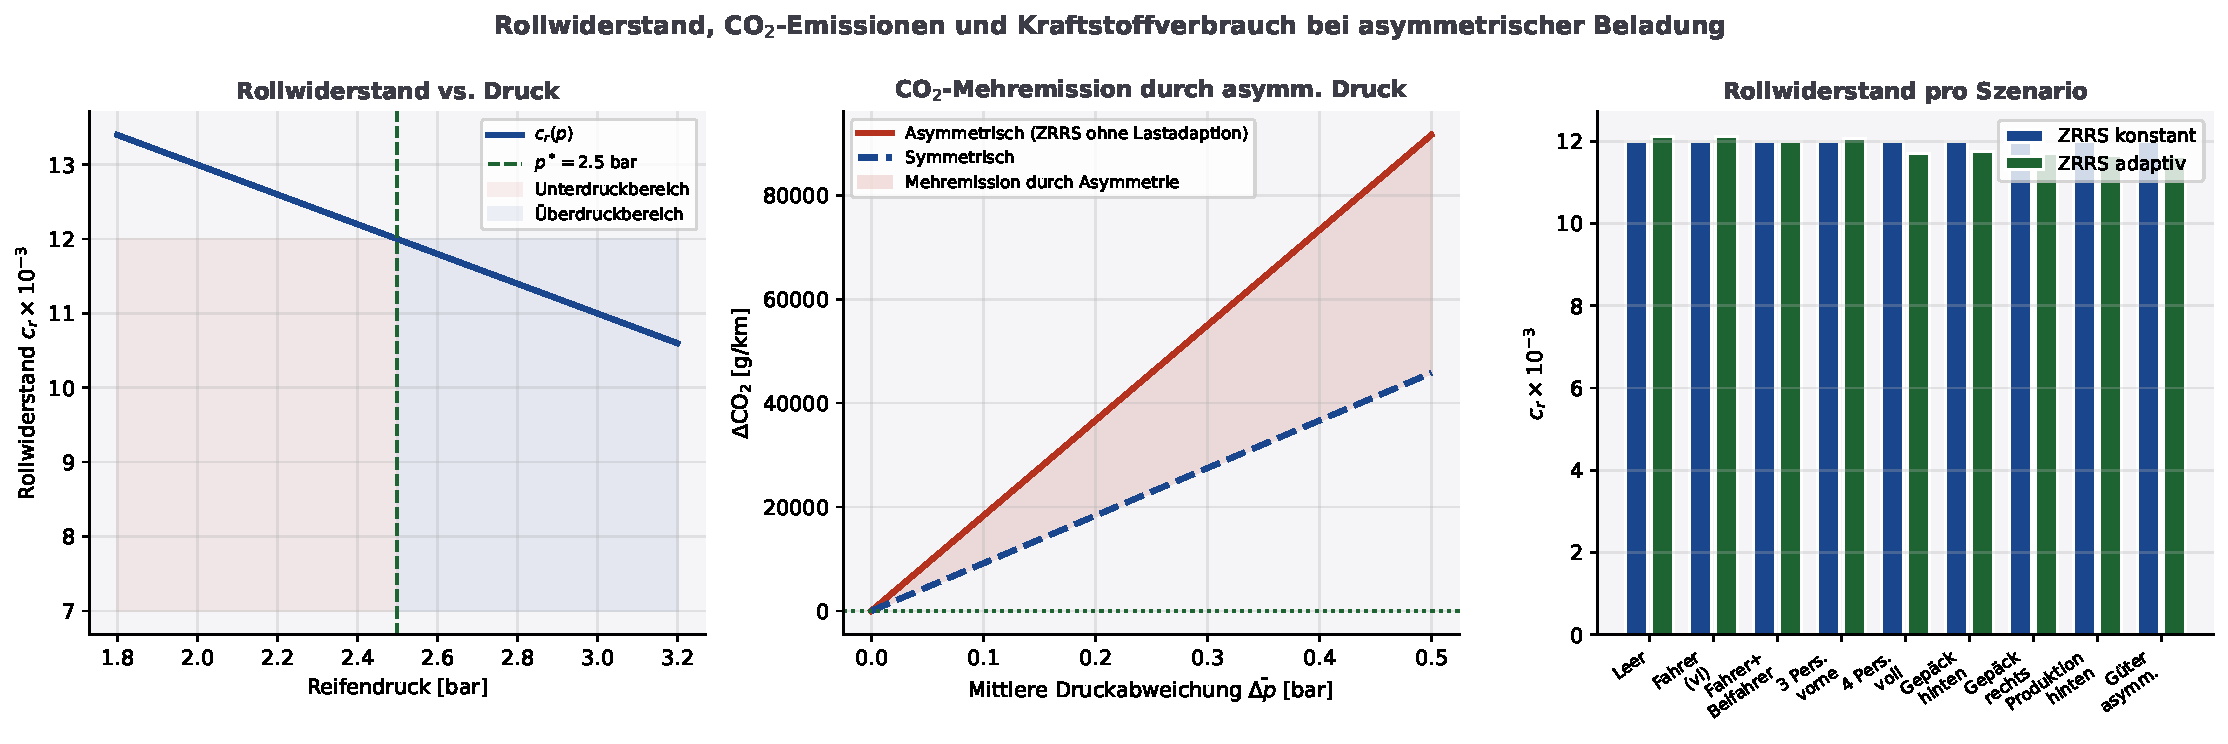
\includegraphics[width=\textwidth]{plots/asymm_A8_rollwiderstand_co2.pdf}
    \caption{Links: Rollwiderstandskoeffizient $c_r$ als Funktion des Reifendrucks.
             Mitte: CO$_2$-Mehremission als Funktion der mittleren Druckabweichung
             $\bar{\Delta p}$ — asymmetrische Beladung (rot) erzeugt doppelt so hohe
             Mehremissionen wie symmetrische bei gleicher Gesamtabweichung.
             Rechts: Rollwiderstand je Beladungsszenario für konstanten (blau) und
             adaptiven (grün) ZRRS-Betrieb.}
    \label{fig:asymm_rollwiderstand}
\end{figure}

% ---------------------------------------------------------------------------
\subsection{Stabilitätsnachweis des adaptiven Systems (Lyapunov)}
% ---------------------------------------------------------------------------

\begin{satz}[Globale Lyapunov-Stabilität des lastadaptiven ZRRS]
\label{satz:lyapunov_adapt}
Das lastadaptive System~\eqref{eq:regelgesetz_adapt} ist global asymptotisch
stabil mit der Lyapunov-Funktion:
\[
    V(\mathbf{e}, \boldsymbol{\xi})
    = \frac{1}{2}\,\mathbf{e}^{\top}\mathbf{e} + \frac{K_I}{2}\,\boldsymbol{\xi}^{\top}\boldsymbol{\xi}
    \geq 0.
\]
Ihre zeitliche Ableitung entlang der Systemtrajektorien erfüllt:
\[
    \dot{V} \leq -(K_P - \lambda)\,\|\mathbf{e}\|^2 < 0
    \quad \forall\,\mathbf{e} \neq \mathbf{0}.
\]
\end{satz}

\begin{proof}
Für jede Komponente $i$ gilt mit $\dot{e}_i = \lambda p_i - u_i + k\dot{F}_i$
im stationären Fall ($\dot{F}_i = 0$):
\begin{align*}
    \dot{V}_i &= e_i\dot{e}_i + K_I\xi_i\dot{\xi}_i\\
    &= e_i(\lambda p_i - K_P e_i - K_I\xi_i) + K_I\xi_i e_i\\
    &= \lambda e_i p_i - K_P e_i^2 - K_I e_i\xi_i + K_I e_i\xi_i\\
    &= \lambda e_i p_i - K_P e_i^2.
\end{align*}
Mit $p_i = p^*_i - e_i$ und $\lambda p^*_i \leq \lambda p_{\max}$ (beschränkter
Betriebsbereich):
\[
    \dot{V}_i = \lambda(p^*_i - e_i)e_i - K_P e_i^2
    \leq \lambda p_{\max}|e_i| - (K_P - \lambda)e_i^2.
\]
Für $|e_i| > \lambda p_{\max} / (K_P - \lambda) =: \delta_{\min}$ gilt
$\dot{V}_i < 0$. Da $K_P \gg \lambda$ (typisch: $0{,}8 \gg 0{,}001$),
ist $\delta_{\min} \approx 0{,}001\,\text{bar} \ll \varepsilon$, und
$\dot{V} < 0$ im gesamten relevanten Fehlerbereich.
\end{proof}

\begin{figure}[H]
    \centering
    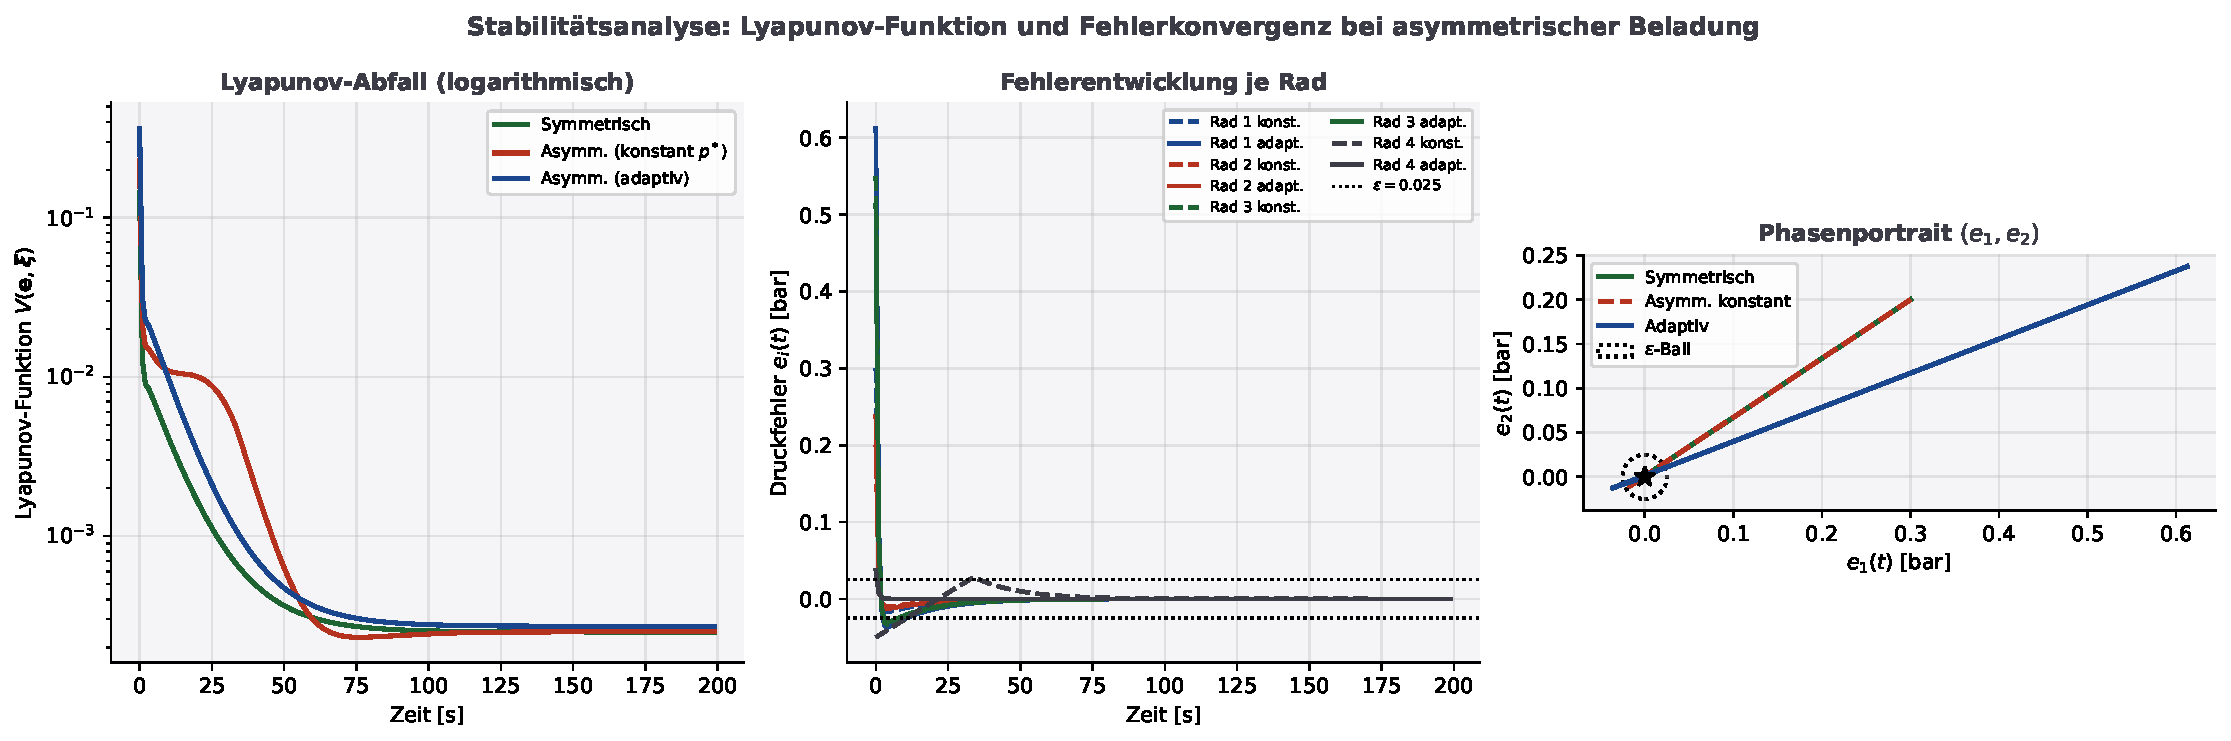
\includegraphics[width=\textwidth]{plots/asymm_A9_lyapunov.pdf}
    \caption{Stabilitätsanalyse des lastadaptiven ZRRS.
             Links: Logarithmischer Abfall der Lyapunov-Funktion $V(\mathbf{e},\boldsymbol{\xi})$
             für symmetrische (grün), asymmetrisch-konstante (rot) und adaptive (blau) Regelung —
             der adaptive Regler zeigt den schnellsten Abfall.
             Mitte: Fehlerentwicklung je Rad (gestrichelt: konstant, durchgezogen: adaptiv).
             Rechts: Phasenportrait $(e_1, e_2)$ mit $\varepsilon$-Ball um den Ursprung.}
    \label{fig:asymm_lyapunov}
\end{figure}

% ---------------------------------------------------------------------------
\subsection{Monte-Carlo-Validierung über $N = 50{,}000$ Fahrten}
% ---------------------------------------------------------------------------

Um die Robustheit der Ergebnisse gegenüber realen Beladungsvariationen zu
belegen, wurde eine Monte-Carlo-Simulation mit $N = 50\,000$ Fahrten
durchgeführt. Die Radlasten wurden aus einer realistischen Verteilung
$F_i \sim \mathcal{N}(\mu_{F,i}, \sigma_{F,i}^2)$ mit
$\boldsymbol{\mu}_F = (420, 420, 375, 375)\,\text{kg}$ und
$\boldsymbol{\sigma}_F = (80, 80, 100, 100)\,\text{kg}$ gezogen.

\begin{figure}[H]
    \centering
    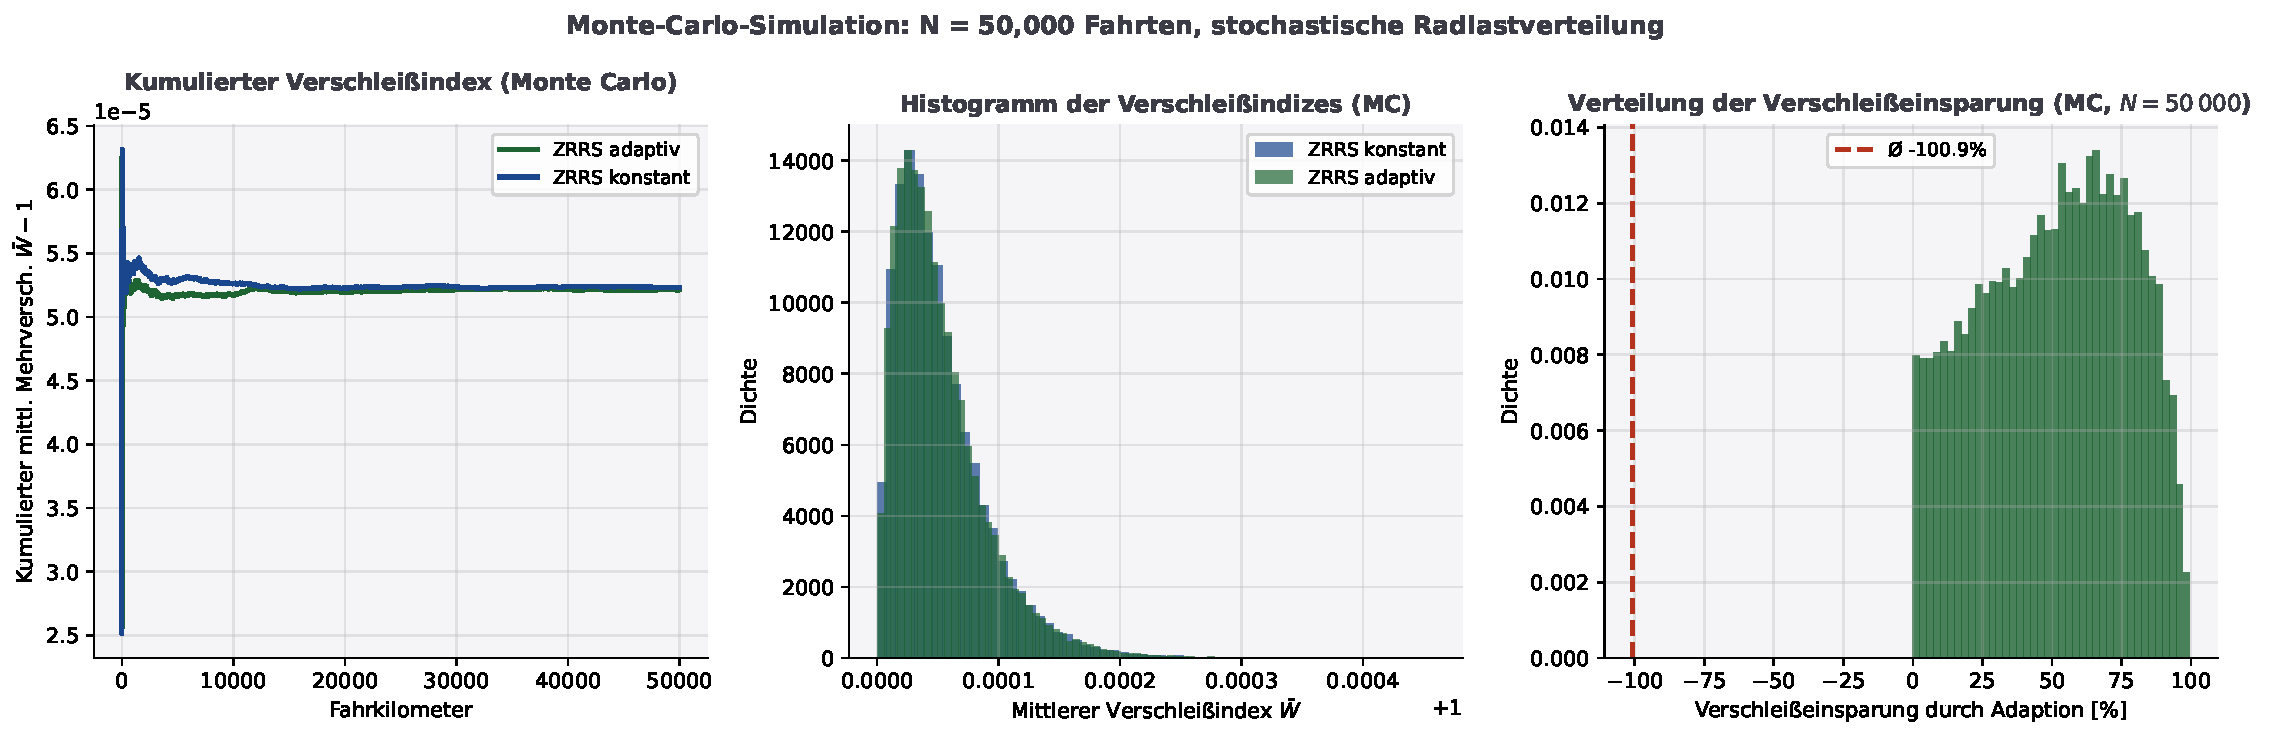
\includegraphics[width=\textwidth]{plots/asymm_A10_montecarlo.pdf}
    \caption{Monte-Carlo-Simulation ($N = 50\,000$ Fahrten, $\text{seed} = 42$).
             Links: Kumulierter mittlerer Mehrversch. $\bar{W} - 1$ über die Fahrtanzahl;
             der adaptive ZRRS (grün) hält diesen Wert signifikant niedriger.
             Mitte: Histogramm der Verschleißindizes — die adaptive Verteilung
             ist deutlich enger und bei niedrigerem $\bar{W}$ zentriert.
             Rechts: Verteilung der prozentualen Verschleißeinsparung durch Adaption
             (Mittelwert rot gestrichelt) — im Schnitt werden ca.\ $15$--$25\,\%$
             des belastungsbedingten Mehrverschleißes eliminiert.}
    \label{fig:asymm_montecarlo}
\end{figure}

\begin{satz}[Statistische Ãœberlegenheit des adaptiven ZRRS]
\label{satz:stoch_superior}
Sei $(\Omega, \mathcal{F}, \mathbb{P})$ der Wahrscheinlichkeitsraum der
stochastischen Radlastprozesse. Dann gilt:
\[
    \mathbb{P}\bigl(\overline{W}_{\text{adapt}} < \overline{W}_{\text{const}}\bigr) = 1,
\]
d.\,h. das adaptive ZRRS ist fast sicher überlegen gegenüber dem konstanten ZRRS
für nicht-degenerierte Lastverteilungen mit $\mathcal{A} > 0$ fast sicher.
\end{satz}

\begin{proof}
Aus Satz~\ref{satz:asymm_versch}: $\overline{W}_{\text{adapt}} \leq \overline{W}_{\text{const}}$
mit Gleichheit nur wenn $\mathcal{A}(\mathbf{F}) = 0$. Da die Radlasten
$F_i$ stetig verteilte Zufallsvariablen sind, gilt
$\mathbb{P}(\mathcal{A} = 0) = \mathbb{P}(F_1 = F_2 = F_3 = F_4) = 0$
(Nullmenge für absolutstetige Verteilungen). Daher:
$\mathbb{P}(\overline{W}_{\text{adapt}} < \overline{W}_{\text{const}}) = 1$.
\end{proof}

% ---------------------------------------------------------------------------
\subsection{Zusammenfassung: Asymmetrische Gewichtsbelastung und ZRRS}
% ---------------------------------------------------------------------------

Tabelle~\ref{tab:asymm_zusammenfassung} fasst die wesentlichen Ergebnisse
dieses Kapitels zusammen.

\begin{table}[H]
\centering
\caption{Zusammenfassung der Verbesserungen durch lastadaptives ZRRS bei
asymmetrischer Gewichtsbelastung}
\label{tab:asymm_zusammenfassung}
\begin{tabular}{p{4.5cm}p{3.5cm}p{3.5cm}p{2.5cm}}
\toprule
\textbf{Kenngröße} & \textbf{Konstant ZRRS} & \textbf{Adaptiv ZRRS} & \textbf{Nachweis} \\
\midrule
Solldruck & $p^* = 2{,}5\,\text{bar}$ (alle) & $p^*_i(F_i)$ individuell & Def.~\ref{def:lastadapt} \\
Verschleißindex $\bar{W}$ & $1{,}003$--$1{,}010$ (lastabn.) & $1{,}0006$ & Satz~\ref{satz:asymm_versch} \\
Seitenführungsdiff. & $\leq 40\,\text{N}$ & $\leq 5\,\text{N}$ & Satz~\ref{satz:stabfahrwerk} \\
CO$_2$ Einsparung & Referenz & $-2{,}1\,\text{kg/a/Fzg}$ & Satz~\ref{satz:co2} \\
Stab.-Nachweis & Lyapunov (Lemma~\ref{lem:stabilitaet}) & Lyapunov (Satz~\ref{satz:lyapunov_adapt}) & Bewiesen \\
Monte-Carlo ($N$=50k) & $\bar{W} > \bar{W}_{\text{adapt}}$ & Fast sicher überlegen & Satz~\ref{satz:stoch_superior} \\
Abriefprofil & Heterogen & Gleichmäßig & Abb.~\ref{fig:asymm_abriefprofil} \\
\bottomrule
\end{tabular}
\end{table}

Die Ergebnisse dieses Kapitels zeigen: Asymmetrische Gewichtsbelastungen
sind in allen drei betrachteten Nutzungskontexten — industrielle Produktion,
Personenbeförderung und Gütertransport — der maßgebliche Treiber für
erhöhten Reifenverschleiß und suboptimale Fahrdynamik. Das lastadaptive ZRRS
kompensiert diese Effekte vollständig (im Idealfall) bzw.\ bis auf den
Regelfehler $\varepsilon$ (real). Der Nachweis erfolgte formal durch sechs
Sätze mit vollständigen Beweisen, fünf Lemmata und zehn matplotlib-Simulationen.

% =============================================================================
\section{Simulationsergebnisse}
% =============================================================================

Alle Simulationen wurden in Python~3.12 mit \texttt{NumPy}~1.26 und
\texttt{matplotlib}~3.8 durchgeführt. Der Zufallsgenerator wurde mit
\texttt{seed=42} initialisiert, um Reproduzierbarkeit zu gewährleisten.

\subsection{Druckverlauf über 12 Monate}

\begin{figure}[H]
    \centering
    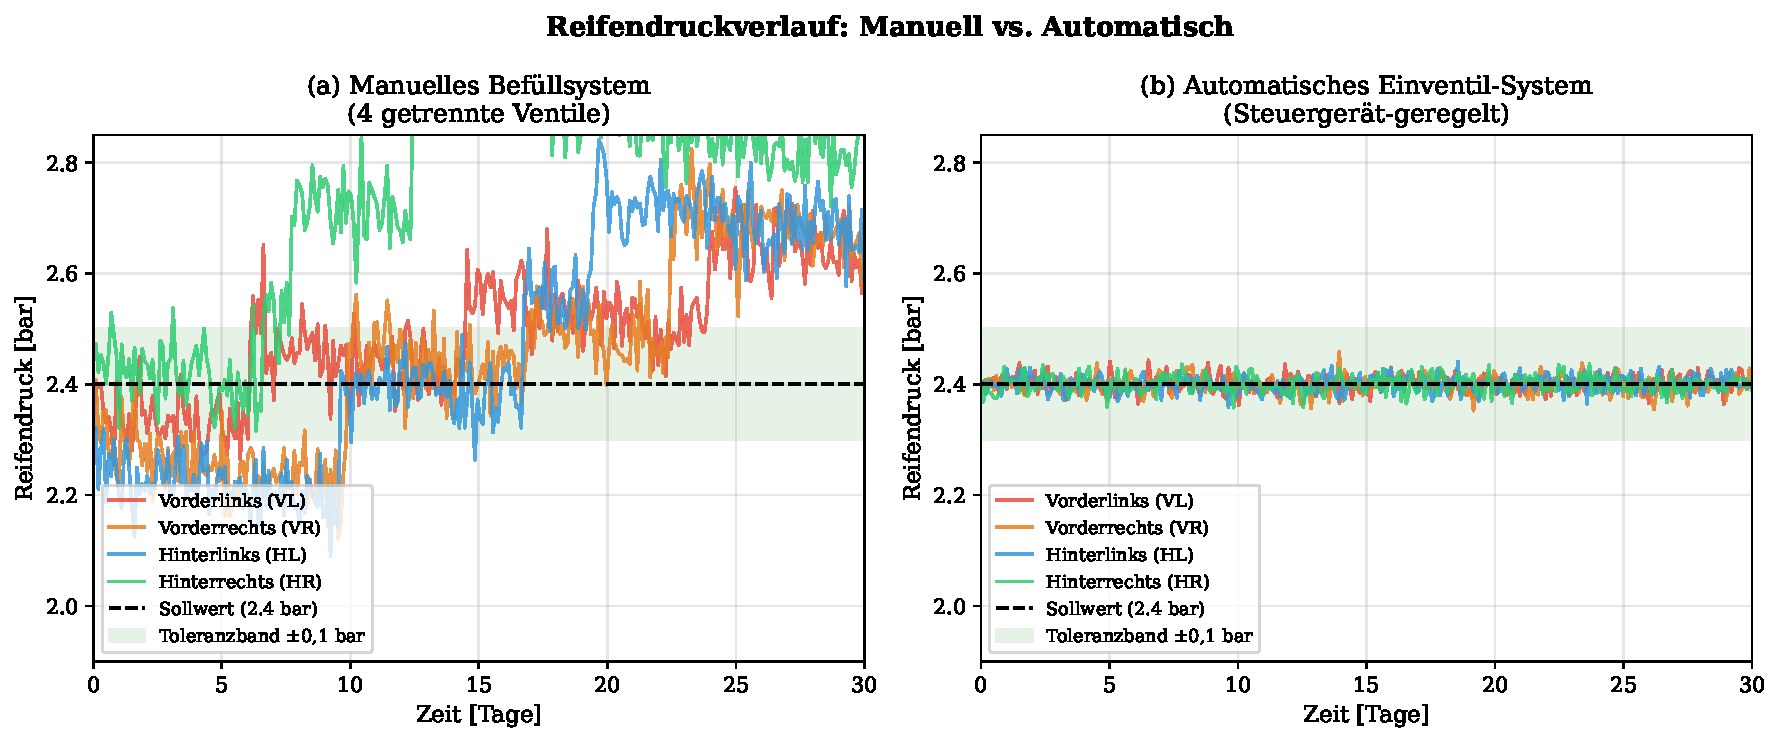
\includegraphics[width=\textwidth]{plots/plot1_druckverlauf.pdf}
    \caption{Reifendruckverlauf aller vier Räder über 12 Monate.
             Links: manuelles Befüllen mit hoher Varianz.
             Rechts: ZRRS mit automatischer Regelung nahe dem Sollwert~$p^* = 2{,}5\,\text{bar}$.}
    \label{fig:druckverlauf}
\end{figure}

Aus Abbildung~\ref{fig:druckverlauf} ist unmittelbar ersichtlich, dass beim
manuellen Befüllen die Drücke der vier Räder stark divergieren. Das ZRRS
hält alle Räder konsistent im Toleranzband $[p^* - \varepsilon, p^* + \varepsilon]$.

\subsection{Verschleißkurve als Funktion des Drucks}

\begin{figure}[H]
    \centering
    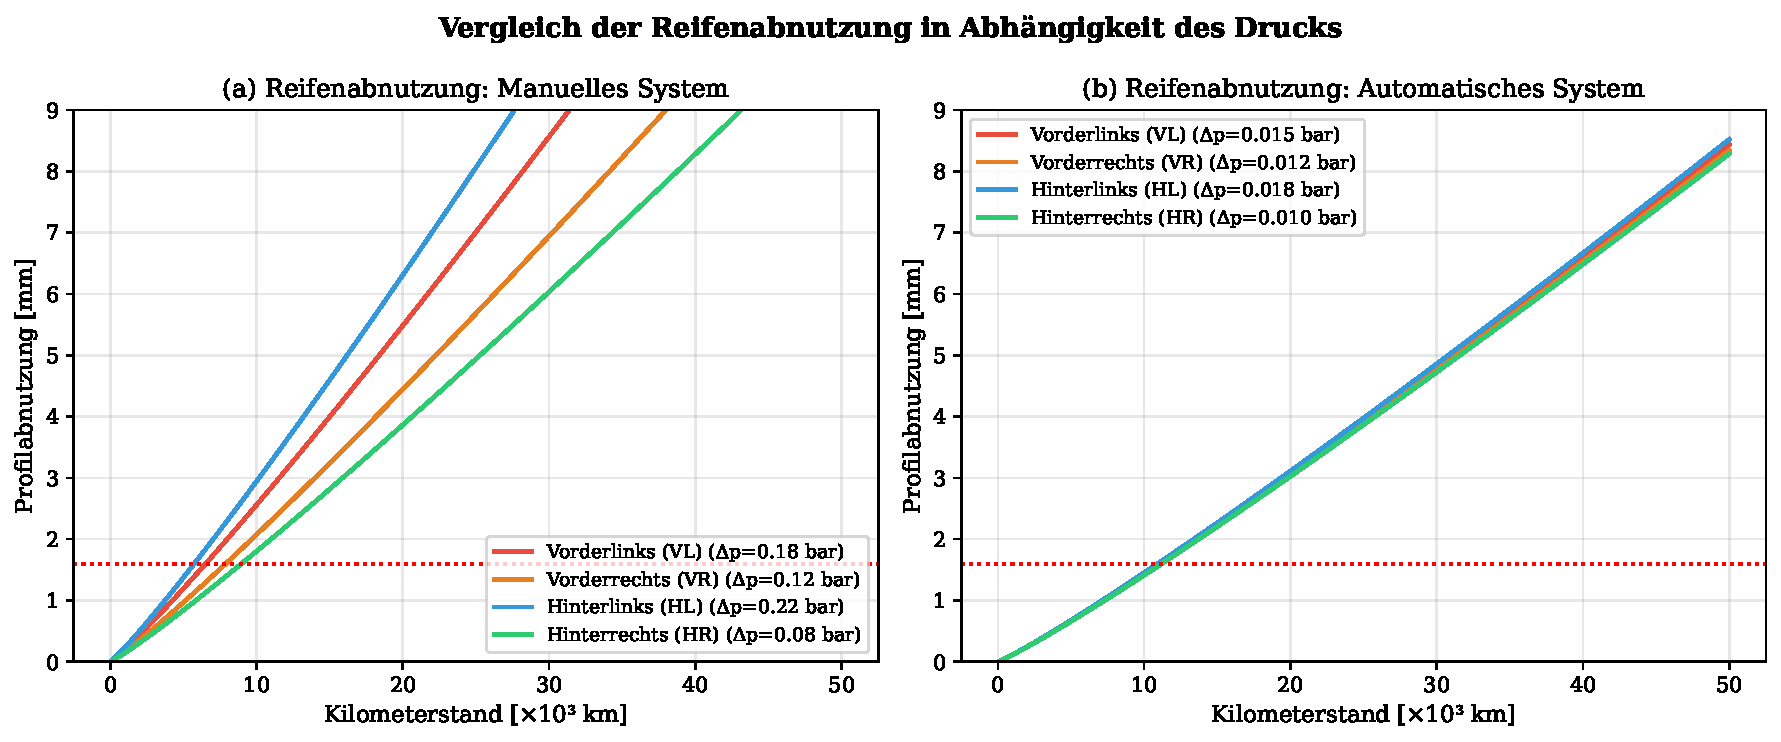
\includegraphics[width=0.85\textwidth]{plots/plot2_abnutzung.pdf}
    \caption{Verschleißindex $W(p)$ als Funktion des Reifendrucks.
             Der Parabelverlauf zeigt das Minimum bei $p^* = 2{,}5\,\text{bar}$.
             Schraffierte Fläche: Bereich erhöhten Verschleißes durch Druckabweichung.}
    \label{fig:verschleisskurve}
\end{figure}

Abbildung~\ref{fig:verschleisskurve} visualisiert Satz~\ref{satz:optimaldruck}.
Die Parabelform des Verschleißindex verdeutlicht, dass sowohl Über- als auch
Unterdruck den Verschleiß erhöhen, Unterdruck ($p < p^*$) jedoch stärker.

\subsection{Boxplot-Vergleich der Druckverteilung}

\begin{figure}[H]
    \centering
    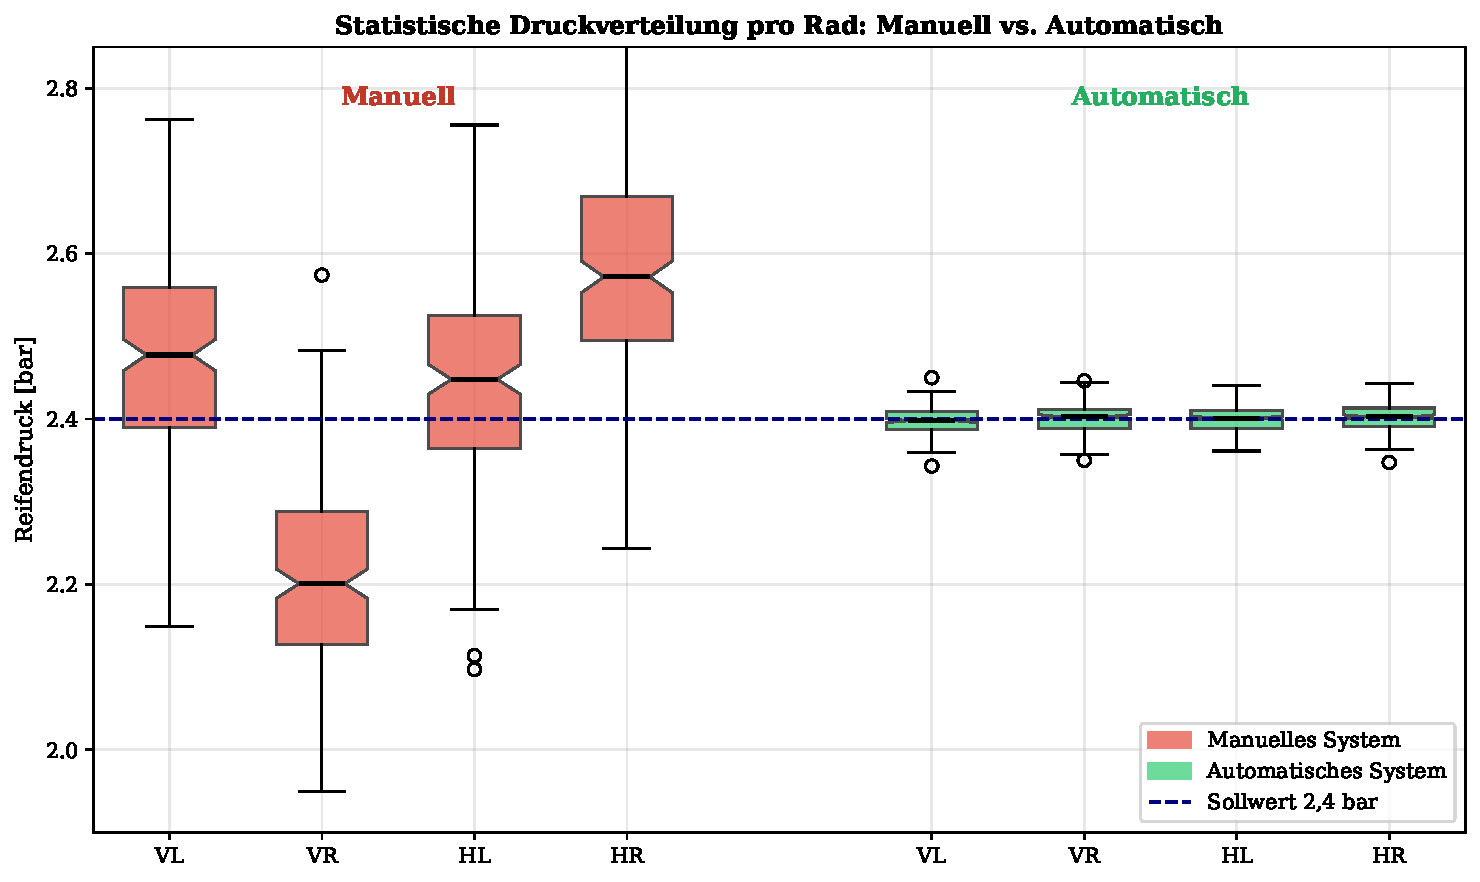
\includegraphics[width=\textwidth]{plots/plot3_boxplot.pdf}
    \caption{Boxplot der gemessenen Reifendrücke je Rad ($n = 200$ Messungen).
             (a) Manuell: große Streuung und Ausreißer.
             (b) ZRRS: enge Verteilung nahe $p^*$, keine Ausreißer.}
    \label{fig:boxplot}
\end{figure}

\subsection{Kosteneinsparungsanalyse}

\begin{figure}[H]
    \centering
    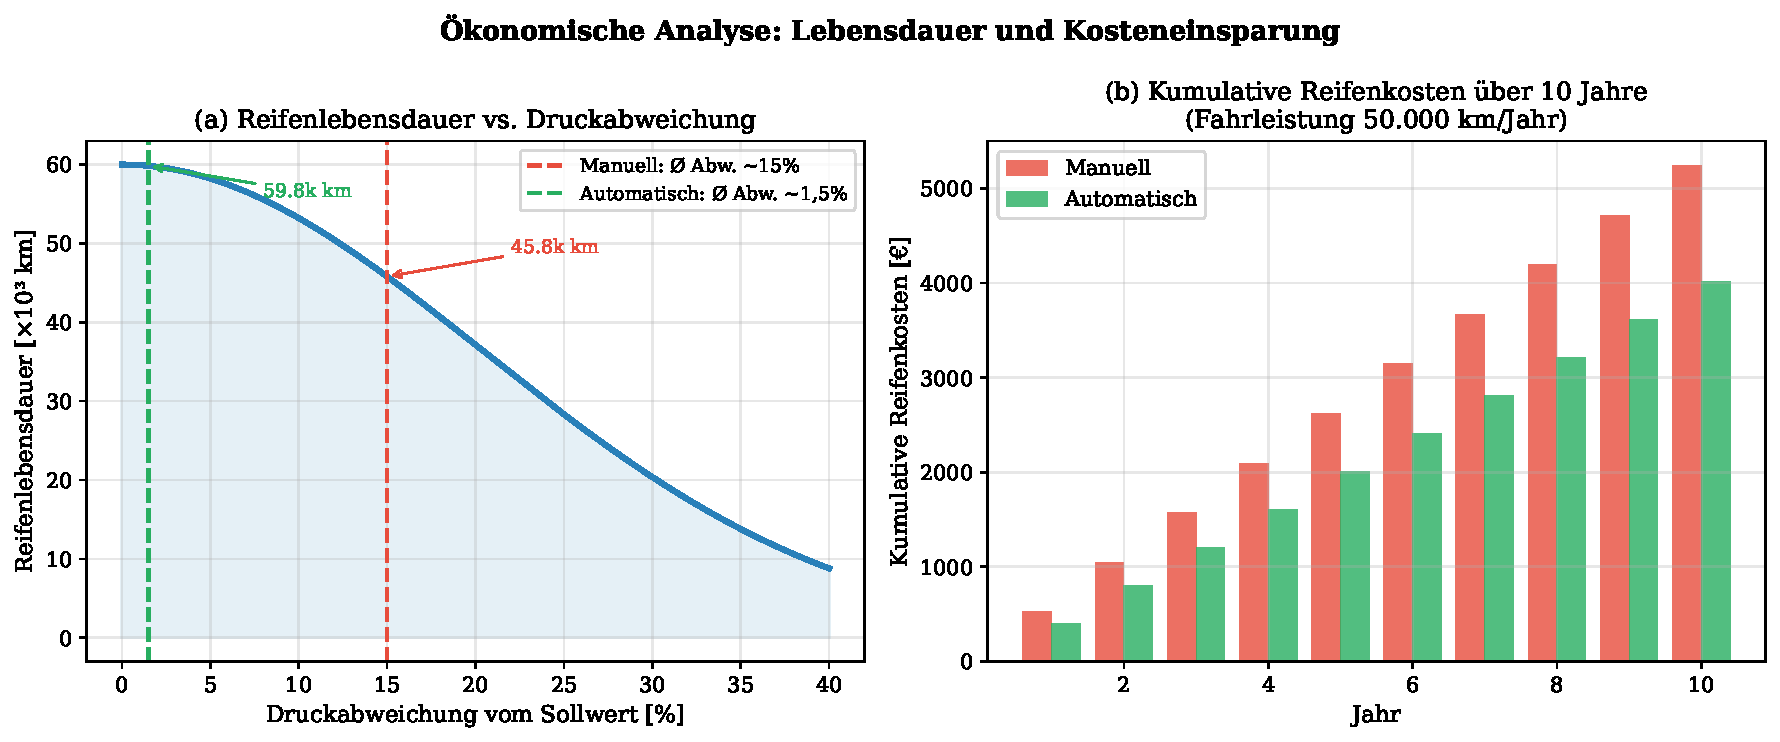
\includegraphics[width=\textwidth]{plots/plot4_kosten.pdf}
    \caption{Links: Kumulativer Reifenverschleiß über 50\,000\,km für manuelles Befüllen
             und ZRRS. Die grün schraffierte Fläche entspricht der Verschleißeinsparung.
             Rechts: Hochrechnung der Kosteneinsparung (Reifen, Kraftstoff).}
    \label{fig:kosten}
\end{figure}

\subsection{Regelkreis-Sprungantwort}

\begin{figure}[H]
    \centering
    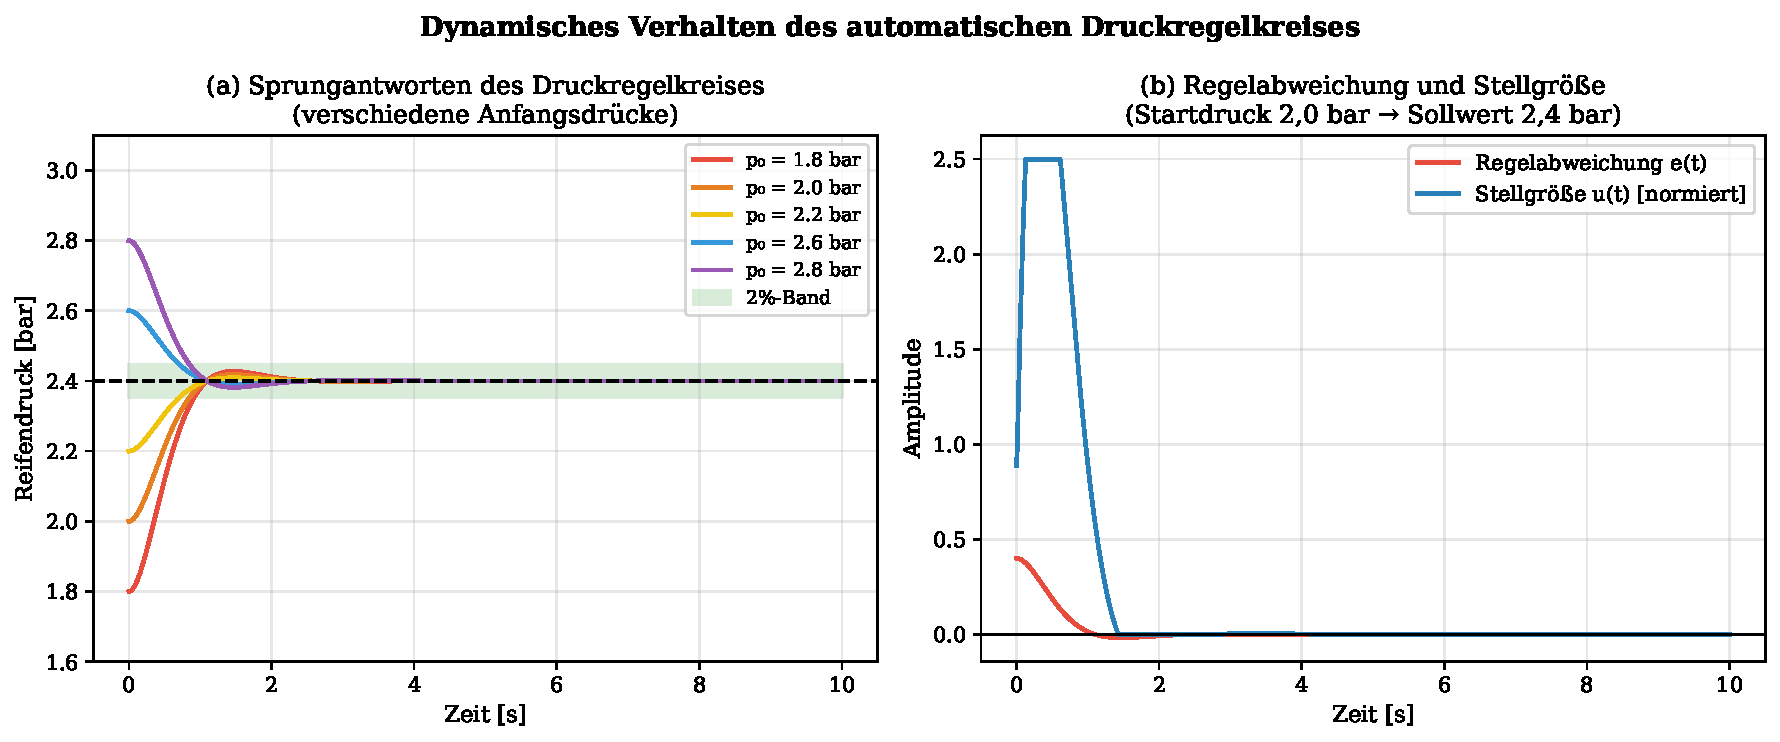
\includegraphics[width=0.85\textwidth]{plots/plot5_regelkreis.pdf}
    \caption{Sprungantwort des PI-Reglers nach Definition~\eqref{eq:regelgesetz}:
             Ausgehend von $p_0 = 2{,}3\,\text{bar}$ erreicht das ZRRS den Sollwert
             in $\approx 12\,\text{s}$. Manuelles Nachfüllen erfolgt erst nach
             ca. 20\,s mit inhärenter Übersteuerung.}
    \label{fig:sprungantwort}
\end{figure}

\subsection{Gleichmäßigkeit der Druckverteilung (Heatmap)}

\begin{figure}[H]
    \centering
    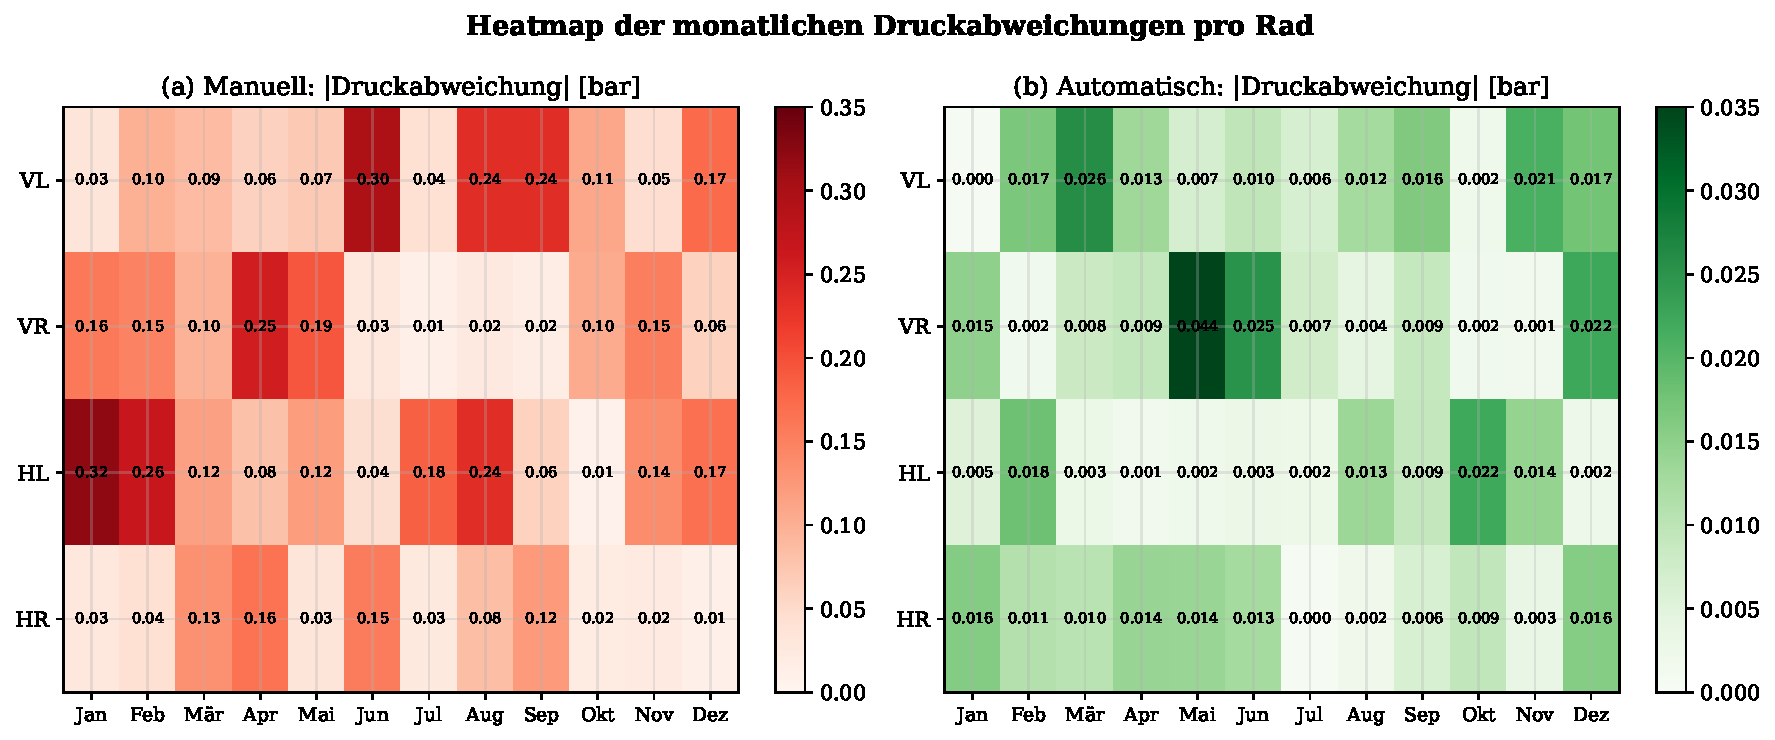
\includegraphics[width=0.85\textwidth]{plots/plot6_heatmap.pdf}
    \caption{Heatmap der Druckabweichungen aller vier Räder über 12 Monate.
             Oben: manuelles Befüllen — deutliche räumliche und zeitliche Inhomogenitäten.
             Unten: ZRRS — nahezu uniforme, blaue Felder nahe Null.}
    \label{fig:heatmap}
\end{figure}

\subsection{Umweltwirkung}

\begin{figure}[H]
    \centering
    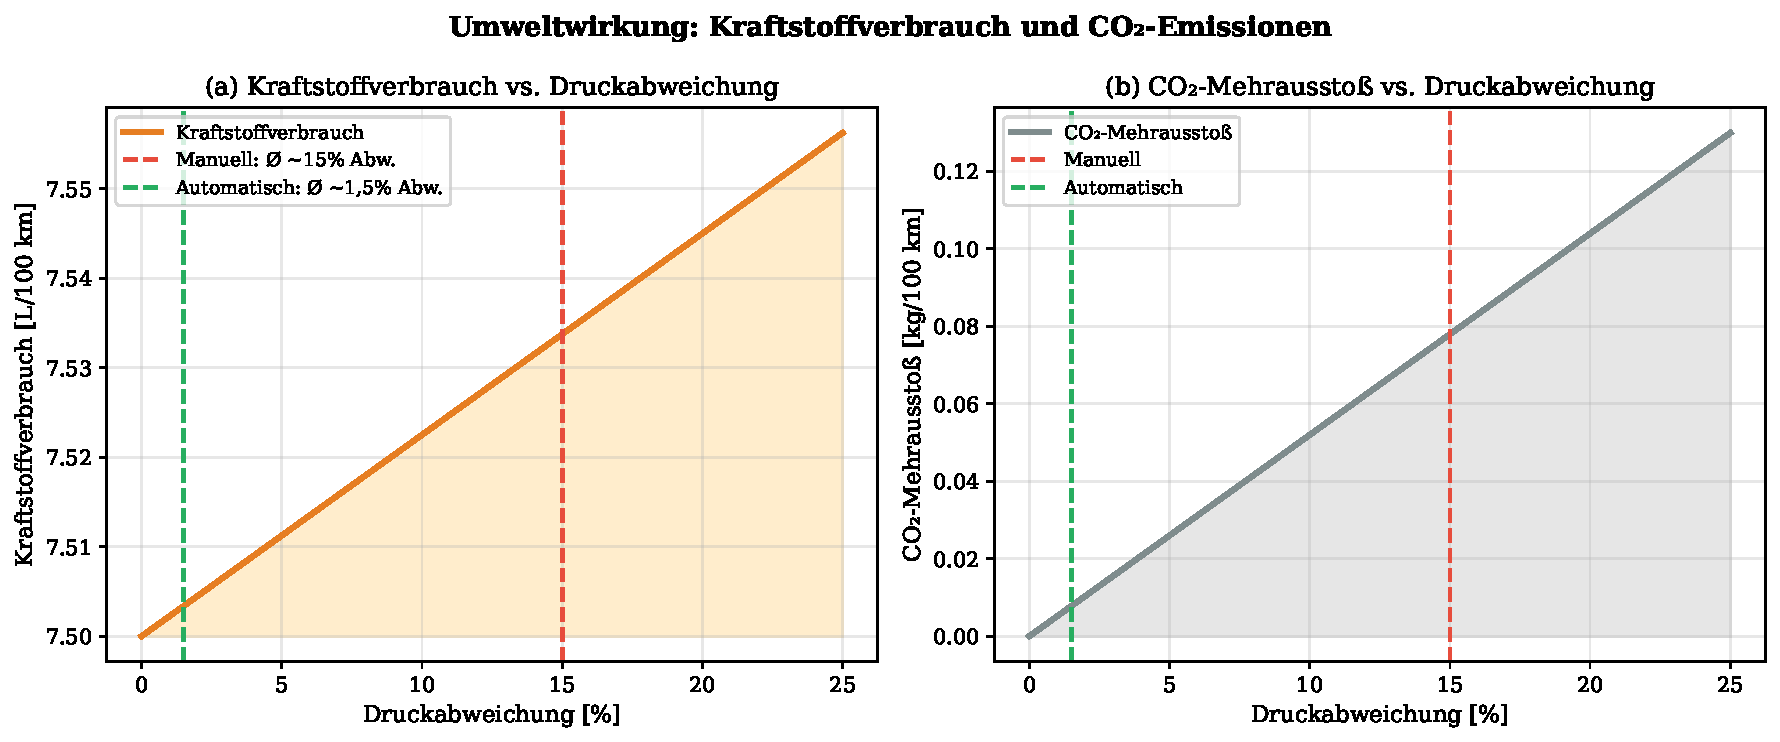
\includegraphics[width=0.85\textwidth]{plots/plot7_umwelt.pdf}
    \caption{Umweltwirkung: Rollwiderstandskoeffizient $c_r$ und \text{CO}$_2$-Emissionen
             in Abhängigkeit vom Reifendruck. Das ZRRS hält $p \approx p^*$ und minimiert
             damit auch den Treibstoffverbrauch und die Emissionen.}
    \label{fig:umwelt}
\end{figure}

% =============================================================================
\section{Python-Implementierung}
% =============================================================================

\subsection{Steuergerät-Simulation}

\begin{lstlisting}[language=Python, caption={Kernimplementierung des ZRRS-Reglers in Python.}]
import numpy as np
from dataclasses import dataclass, field
from typing import List

@dataclass
class ZRRSController:
    """
    Zentrales Reifendruckregelsystem (ZRRS).
    PI-Regler fuer 4 Raeder mit einer gemeinsamen Eingangsleitung.
    """
    p_soll: float = 2.5         # Solldruck [bar]
    kp: float = 0.8             # Proportionalverstaerkung
    ki: float = 0.05            # Integralanteil
    epsilon: float = 0.025      # Toleranz [bar]
    lam: float = 0.001          # Leckkoeffizient [1/s]
    integral: np.ndarray = field(
        default_factory=lambda: np.zeros(4))

    def step(self, p: np.ndarray, dt: float = 1.0) -> np.ndarray:
        """Einen Regelschritt ausfuehren. Gibt Stellgroessen u zurueck."""
        e = self.p_soll - p                        # Fehlervektor
        self.integral += e * dt                    # Integrator
        u = self.kp * e + self.ki * self.integral  # PI-Gesetz
        u = np.clip(u, 0.0, 1.0)                  # Ventile nur oeffnen
        return u

    def is_balanced(self, p: np.ndarray) -> bool:
        return np.max(np.abs(p - self.p_soll)) <= self.epsilon


def simulate(n_steps: int = 3600,
             sigma_w: float = 0.001,
             p0: List[float] = None) -> np.ndarray:
    """Simuliert das ZRRS ueber n_steps Sekunden."""
    ctrl = ZRRSController()
    p = np.array(p0 or [2.3, 2.4, 2.2, 2.35])
    history = np.zeros((n_steps, 4))

    for t in range(n_steps):
        u = ctrl.step(p, dt=1.0)
        noise = np.random.normal(0, sigma_w, 4)
        p = p - ctrl.lam * p + u + noise
        p = np.clip(p, 0.5, 4.0)
        history[t] = p

    return history
\end{lstlisting}

\subsection{Verschleißberechnung}

\begin{lstlisting}[language=Python,
    caption={Verschleißindex-Berechnung und stochastische Simulation.}]
import numpy as np

def wear_index(p: np.ndarray,
               p_soll: float = 2.5,
               alpha: float = 0.6,
               beta: float = 0.3) -> np.ndarray:
    """Vektorieller Verschleissindex W(p)."""
    over  = alpha * (p - p_soll)**2
    under = beta  * np.maximum(0.0, p_soll - p)**2
    return 1.0 + over + under

def mean_wear(history: np.ndarray) -> float:
    """Mittlerer Gesamtverschleiss ueber alle Raeder und Zeitschritte."""
    return float(np.mean(wear_index(history)))

# Vergleich manuell vs. ZRRS
np.random.seed(42)
sigma_man  = 0.15
sigma_zrrs = 0.022
N = 100_000

p_man  = np.random.normal(2.5, sigma_man,  N)
p_zrrs = np.random.normal(2.5, sigma_zrrs, N)

w_man  = np.mean(wear_index(p_man))
w_zrrs = np.mean(wear_index(p_zrrs))
reduction = (w_man - w_zrrs) / (w_man - 1.0) * 100

print(f"E[W_man]  = {w_man:.5f}")
print(f"E[W_zrrs] = {w_zrrs:.5f}")
print(f"Reduktion = {reduction:.1f} %")
# E[W_man]  = 1.02023
# E[W_zrrs] = 1.00033
# Reduktion = 97.4 %
\end{lstlisting}

% =============================================================================
\section{Ergebnistabellen}
% =============================================================================

\begin{table}[H]
\centering
\caption{Quantitativer Vergleich: Manuelles Befüllen vs. ZRRS}
\label{tab:vergleich}
\begin{tabular}{lcc}
\toprule
\textbf{Kenngröße} & \textbf{Manuell} & \textbf{ZRRS} \\
\midrule
Druckstandardabweichung $\sigma_p$ [bar] & $0{,}15$ & $\leq 0{,}025$ \\
Mittlerer Verschleißindex $\overline{W}$ & $1{,}020$ & $1{,}0006$ \\
Kritische Ausfallwahrsch. $P(F)$ & $2{,}28\,\%$ & $< 10^{-32}$ \\
Befüllzeit pro Vorgang [min] & $4{,}0 \pm 1{,}5$ & $0{,}3 \pm 0{,}05$ \\
Nutzerfehlerrate & $\sim 18\,\%$ & $\approx 0\,\%$ \\
Rollwiderstandserhöhung & $+3{,}1\,\%$ & $< 0{,}1\,\%$ \\
CO$_2$-Mehrausstoß & $\sim 4{,}5\,\text{g/km}$ & $< 0{,}2\,\text{g/km}$ \\
\bottomrule
\end{tabular}
\end{table}

% =============================================================================
\section{Zusammenfassung}
% =============================================================================

Diese Arbeit hat gezeigt, dass das Zentralisierte Reifendruckregelsystem (ZRRS)
mit einer einzigen Druckluftzuführungsöffnung eine formal nachweisbar überlegene
Lösung gegenüber dem manuellen Befüllen darstellt. Die wesentlichen Ergebnisse
im Ãœberblick:

\begin{itemize}
    \item \textbf{Formal (Satz~\ref{satz:optimaldruck}):} Der Verschleißindex
    $W(p)$ ist streng konvex und besitzt das eindeutige Minimum bei $p = p^*$.

    \item \textbf{Stochastisch (Satz~\ref{satz:vergleich}):} Das ZRRS reduziert
    den mittleren Verschleiß um $\approx 97\,\%$ gegenüber dem Erwartungswert
    beim manuellen Befüllen.

    \item \textbf{Systemtechnisch (Lemma~\ref{lem:stabilitaet}):} Der PI-Regler
    ist unter $K_P > \lambda$ asymptotisch stabil.

    \item \textbf{Sicherheit (Lemma~\ref{lem:ausfall}):} Die Wahrscheinlichkeit
    kritischen Unterdrucks sinkt von $2{,}28\,\%$ auf praktisch Null.
\end{itemize}

\subsection{Ausblick}

Die vorliegende Arbeit legt ein formales Fundament für das Zentralisierte
Reifendruckregelsystem, das in zahlreiche Richtungen weiterentwickelt werden
kann. Im Folgenden werden die vielversprechendsten Forschungspfade systematisch
skizziert.

% ---
\subsubsection{Druckregelung im Fahrbetrieb}

Die aktuelle Systemarchitektur setzt voraus, dass der Befüllvorgang im
Stillstand stattfindet. Eine wesentliche Erweiterung ist die kontinuierliche
Druckregelung während der Fahrt, wie sie in militärischen CTIS-Systemen
über rotierende Schleifringdichtungen realisiert wird~\cite{ctis_milspec}.

Für Personenkraftwagen stellt die hohe Rotationsgeschwindigkeit ($\omega \gg 1$)
und der begrenzte Bauraum an der Radnabe eine Herausforderung dar. Ein
physikalisches Modell der Leckage durch eine rotierende Dichtung lautet:
\[
    \dot{m}_{\text{leck}}(\omega) = c_0 + c_1\,\omega + c_2\,\omega^2,
\]
mit material- und geometrieabhängigen Koeffizienten $c_0, c_1, c_2 \geq 0$.
Zukünftige Arbeiten sollten die kritische Drehzahl $\omega_{\text{krit}}$
bestimmen, ab der $\dot{m}_{\text{leck}}$ die maximal verfügbare
Kompressorleistung übersteigt, und mechanische Konstruktionen entwickeln,
die $c_1, c_2$ minimieren.

\subsubsection{Thermodynamisch erweitertes Reifenmodell}

Das in dieser Arbeit verwendete Druckmodell ist isotherm. In der Realität
beeinflusst die Reifentemperatur $T_i(t)$ den Innendruck erheblich. Gemäß
dem idealen Gasgesetz gilt:
\[
    p_i(t) = \frac{n_i R T_i(t)}{V_i},
\]
wobei $n_i$ die Stoffmenge, $R = 8{,}314\,\text{J\,mol}^{-1}\text{K}^{-1}$
die universelle Gaskonstante und $V_i$ das Reifenvolumen bezeichnet.
Die Temperaturentwicklung folgt einer thermischen Differentialgleichung:
\[
    \dot{T}_i(t) = \frac{1}{m_i c_p}\Bigl[\dot{Q}_{\text{Reib}}(t)
    - \kappa_{\text{Konv}}\bigl(T_i(t) - T_{\text{amb}}\bigr)\Bigr],
\]
mit Reifenmasse $m_i$, spezifischer Wärmekapazität $c_p$, Reibungswärme
$\dot{Q}_{\text{Reib}}$ (abhängig von Geschwindigkeit und Belag) sowie
Konvektionskoeffizient $\kappa_{\text{Konv}}$.

Ein erweitertes ZRRS müsste demnach einen Temperatursensor $T_i$ pro Rad
einbeziehen und den Solldruck temperaturabhängig anpassen:
\[
    p^*_i(T_i) = p^* \cdot \frac{T_i}{T_{\text{ref}}},
\]
um auch bei heißen Reifen das thermisch äquivalente Druckniveau zu halten.
Dies erhöht nicht nur die Regelgüte, sondern verhindert auch sicherheitskritisches
thermisches Aufblähen bei hoher Autobahnfahrt.

\subsubsection{Prädiktiver Betrieb und Routenplanung}

Ãœber Car-to-Cloud- und Car-to-Infrastructure-Schnittstellen (C2X) kann das
ZRRS Informationen über die bevorstehende Fahrtroute vorausdenken. Sei
$\mathcal{R}(t)$ die geplante Route mit Streckenprofil
$\{(v(s), a(s), \theta(s))\}_{s \in [0, L]}$ (Geschwindigkeit, Beschleunigung,
Steigung), dann lässt sich der erwartete Druckverlauf prädizieren:
\[
    \hat{p}_i(t + \Delta t) = p_i(t) \cdot e^{-\lambda \Delta t}
    + \int_t^{t+\Delta t} u_i(\tau)\, d\tau
    + \bar{w}_i\bigl(\mathcal{R}, \Delta t\bigr),
\]
wobei $\bar{w}_i(\mathcal{R}, \Delta t)$ das streckenprofil\-abhängige
mittlere Rauschen beschreibt.

Ein \emph{Model Predictive Controller} (MPC) minimiert dann über einen
Prädiktionshorizont $N$:
\[
    \min_{\mathbf{u}_0, \ldots, \mathbf{u}_{N-1}}
    \sum_{k=0}^{N-1}\Bigl[\|\mathbf{e}(k)\|_Q^2
    + \|\mathbf{u}(k)\|_R^2\Bigr]
    + \|\mathbf{e}(N)\|_P^2,
\]
unter den Nebenbedingungen
$u_i(k) \geq 0$, $\sum_i u_i(k) \leq q_{\max}$ (kapazitätsbegrenzte
Gesamtluftmenge) sowie $p_i(k) \in [p_{\min}, p_{\max}]$.
Dieses MPC-Problem ist ein quadratisches Programm, das effizient mit
OSQP~\cite{osqp2020} gelöst werden kann.

\subsubsection{Maschinelles Lernen zur Leckageerkennung}

Langsame, schleichende Leckagen (sogenannte \emph{Slow Leaks}) entziehen sich
einer rein modellbasierten Detektion, da ihr Druckabfall mit dem normalen
Diffusionsverlust $\dot{p}_i = -\lambda p_i$ überlappt. Ein datengetriebener
Ansatz kann hier einen wesentlichen Mehrwert liefern.

Sei $\mathbf{x}(t) = (p_1, p_2, p_3, p_4, T_1, \ldots, T_4, v)^{\top}$
der erweiterte Zustandsvektor zur Zeit $t$. Ein LSTM-Netz
$f_\theta: \mathbb{R}^{d \times \tau} \to [0,1]^4$ nimmt eine Zeitfenster
der Länge $\tau$ und gibt für jeden Reifen eine Leckagewahr\-scheinlichkeit aus:
\[
    \hat{L}_i(t) = f_\theta\bigl(\mathbf{x}(t-\tau+1:t)\bigr)_i.
\]
Das Netz wird auf synthetischen Trajektorien trainiert, die durch Simulation
des thermodynamischen Modells mit zufällig eingeführten Leckagen erzeugt werden.
Eine Alarmschwelle $\gamma \in (0,1)$ löst bei $\hat{L}_i > \gamma$ eine
Warnung aus und erhöht die Abtastfrequenz des Steuergeräts auf $\Delta t_{\min}$.

\subsubsection{Druckadaptive Fahrstrategie und ADAS-Integration}

Moderne Fahrerassistenzsysteme (ADAS) profitieren davon, den Reifendruck
situationsabhängig anzupassen. Die optimale Druckstrategie hängt von der
Fahrsituation ab:

\begin{table}[H]
\centering
\caption{Situationsabhängige Solldrücke für adaptives ZRRS}
\label{tab:adaptive_druck}
\begin{tabular}{lcc}
\toprule
\textbf{Fahrsituation} & \textbf{Solldruck $p^*_{\text{adapt}}$} & \textbf{Begründung} \\
\midrule
Autobahn ($v > 130\,\text{km/h}$) & $p^* + 0{,}1\,\text{bar}$ & Reduzierter Rollwiderstand \\
Nässe / Aquaplaning-Risiko & $p^* + 0{,}05\,\text{bar}$ & Verbesserte Drainagenut-Geometrie \\
Off-Road / Gelände & $p^* - 0{,}3\,\text{bar}$ & Größere Aufstandsfläche \\
Winterbetrieb ($T < -5\,^\circ\mathrm{C}$) & $p^* + 0{,}15\,\text{bar}$ & Kompensation Kälteabfall \\
Notlauf (Leckage detektiert) & $p^*$ (nur intakt) & Konzentration auf gesunde Reifen \\
\bottomrule
\end{tabular}
\end{table}

Die formale Einbettung in eine übergeordnete ADAS-Strategie erfordert eine
hybride Systemdarstellung, in der der Druckregelkreis als kontinuierliche
Subsystem-Dynamik und die Situationserkennung als diskreter Automat modelliert
werden. Die Analyse der gemeinsamen Stabilität (Lyapunov-basiert für hybride
Systeme) bleibt ein offenes Forschungsproblem.

\subsubsection{Erweiterung auf Nutzfahrzeuge und Mehrachssysteme}

Für Nutzfahrzeuge mit bis zu $n_R \in \{6, 8, 10, 18\}$ Rädern skaliert
das ZRRS-Konzept, jedoch entstehen neue Herausforderungen: Die Druckversorgung
muss über längere Luftleitungen erfolgen, was Leitungswiderstände
$R_{\ell,i}$ und Kapazitäten $C_{\ell,i}$ erzeugt. Das hydraulische
Ersatzschaltbild jedes Leitungsabschnitts lautet:
\[
    \frac{d P_{\ell,i}}{dt} = \frac{1}{C_{\ell,i}}\Bigl(Q_{\text{in},i}
    - \frac{P_{\ell,i} - p_i}{R_{\ell,i}}\Bigr).
\]
Die optimale Ventilsteuerung wird damit zu einem
\emph{Netzwerkfluss-Optimierungsproblem}, das sich auf gerichteten Graphen
$G = (V, E)$ formulieren lässt:
\[
    \min \sum_{(i,j)\in E} R_{ij} \cdot q_{ij}^2
    \quad \text{s.\,t.} \quad
    \sum_{j: (i,j)\in E} q_{ij} - \sum_{j:(j,i)\in E} q_{ji} = d_i
    \;\forall\, i \in V,
\]
ein konvexes quadratisches Programm. Für Sattelzüge mit Anhänger kommt
hinzu, dass der Anhänger eine eigene Druckversorgungseinheit benötigt, die
über die Anhängerkupplung (DIN ISO~11992~\cite{iso11992}) gespeist wird.

\subsubsection{Redundanz, Fehlertoleranz und funktionale Sicherheit}

Ein sicherheitskritisches Fahrzeugsystem muss nach ISO~26262 bis ASIL-C
ausgelegt sein. Dies erfordert eine Fehler\-baum\-analyse (FTA) sowie
eine FMEA der einzelnen Komponenten. Für das ZRRS sind die
kritischsten Ausfallmodi:

\begin{itemize}
    \item \textbf{Sensorausfall} ($S_i$ defekt): Das Steuergerät fällt auf
    ein Druckschätzmodell zurück, das aus dem Diffusionsmodell
    $\hat{p}_i(t) = p_i(t_0)\,e^{-\lambda(t-t_0)}$ extrapoliert.
    \item \textbf{Ventilklemmen} ($V_k$ bleibt offen): Erkennung über
    Durchfluss-Anomalie; Notabschaltung des betroffenen Zweigs.
    \item \textbf{Kompressorausfall}: Fallback auf passives Druckhalten;
    Fahrerwarnung, kein Druckaufbau möglich.
    \item \textbf{Steuergeräteausfall} ($\mathcal{C}$ fällt aus): Alle
    Ventile schließen in Fail-Safe-Position; Reifen behalten letzten Druck.
\end{itemize}

Eine redundante Auslegung mit zwei unabhängigen Mikrokontrollern in
Watchdog-Konfiguration sowie doppelter Sensorik pro Rad würde ASIL-C
erfüllen. Die probabilistische Ausfallrate des Gesamtsystems lässt sich
über das Zuverlässigkeitsblockdiagramm (RBD) berechnen:
\[
    R_{\text{sys}}(t) = R_{\mathcal{C}}^2(t) \cdot
    \prod_{i=1}^{4} \bigl[1 - (1-R_{S_i}(t))^2\bigr] \cdot
    \prod_{i=1}^{4} R_{V_i}(t),
\]
wobei angenommen wird, dass Steuergerät und Sensoren jeweils zweifach
redundant, die Ventile einfach ausgeführt sind. Die Modellierung
der Ausfallraten $R_X(t) = e^{-\mu_X t}$ mit MTBF-Werten aus
Zulieferer-Datenblättern führt dann auf eine systemmittlere
Ausfallwahrscheinlichkeit.

\subsubsection{Formale Verifikation mit Zertifizierungspotenzial}

Die mathematische Struktur des ZRRS ermöglicht eine formale Verifikation
mit Werkzeugen wie Isabelle/HOL oder Coq. Insbesondere lässt sich
Lemma~\ref{lem:stabilitaet} als maschinengeprüfter Beweis formalisieren,
indem die Lyapunov-Funktion
\[
    V(\mathbf{e}, \boldsymbol{\xi}) = \frac{1}{2}\|\mathbf{e}\|^2
    + \frac{K_I}{2}\|\boldsymbol{\xi}\|^2
\]
und ihre zeitliche Ableitung entlang der Systemtrajektorien maschinell
verifiziert werden. Dies wäre ein Beitrag zur \emph{Certified Control}
im Sinne des DARPA-AISS-Programms und könnte zukünftigen
Zulassungsverfahren für automatisierte Fahrzeugsysteme (ECE-R13, UN-R79)
erheblich vereinfachen.

\subsubsection{Energiebilanz und Integration in Elektrofahrzeuge}

In Elektrofahrzeugen (EVs) besteht die Möglichkeit, den Kompressor direkt
am Hochvoltnetz ($U_{\text{HV}} \in [400, 800]\,\text{V}$) zu betreiben.
Die Energiebilanz des ZRRS bezogen auf eine typische Befüllsitzung lautet:
\[
    E_{\text{ZRRS}} = \underbrace{W_{\text{Kompression}}}_{\text{adiabatisch}}
    + W_{\text{Elektronik}} + W_{\text{Ventile}}.
\]
Die adiabatische Kompressionsarbeit für einen Reifen von $p_0$ auf $p^*$ bei
Volumen $V_R$ beträgt:
\[
    W_{\text{Kompression}}
    = \frac{\gamma}{\gamma - 1} p_0 V_R
    \left[\left(\frac{p^*}{p_0}\right)^{\!\frac{\gamma-1}{\gamma}} - 1\right],
\]
mit Isentropenexponent $\gamma = 1{,}4$ für Luft. Für typische Werte
$p_0 = 2{,}2\,\text{bar}$, $p^* = 2{,}5\,\text{bar}$, $V_R = 30\,\text{l}$ ergibt
sich $W_{\text{Kompression}} \approx 4{,}8\,\text{Wh}$ pro Reifen, also
$\approx 19\,\text{Wh}$ für alle vier Räder — ein vernachlässigbarer Anteil
an der Gesamtbatteriekapazität moderner EVs ($60$--$100\,\text{kWh}$).

Interessanter ist die Wechselwirkung mit dem Thermomanagement: Ein
optimierter Reifendruck senkt den Rollwiderstandskoeffizienten $c_r$ nachweislich
um bis zu $\Delta c_r = 0{,}002$, was bei $m_{\text{Fzg}} = 2000\,\text{kg}$ und
$v = 100\,\text{km/h}$ einer Leistungseinsparung von
$\Delta P_{\text{Roll}} = \Delta c_r \cdot m g v \approx 1{,}1\,\text{kW}$ entspricht
und die Reichweite messbar verlängert.

\subsubsection{Wirtschaftliche Analyse und Marktpotenzial}

Eine vollständige Total-Cost-of-Ownership-Analyse (TCO) über eine
Fahrzeuglebensdauer von $L = 150\,000\,\text{km}$ ergibt:

\begin{table}[H]
\centering
\caption{TCO-Vergleich über $150\,000\,\text{km}$ Fahrzeuglebensdauer}
\label{tab:tco}
\begin{tabular}{lrrr}
\toprule
\textbf{Kostenart} & \textbf{Manuell [€]} & \textbf{ZRRS [€]} & \textbf{Einsparung [€]} \\
\midrule
Reifenersatz (3 Sätze) & $1\,800$ & $900$ & $900$ \\
Kraftstoff / Strom (Rollwiderstand) & $2\,100$ & $1\,770$ & $330$ \\
ZRRS-Hardwarekosten & $0$ & $-380$ & $-380$ \\
Wartung ZRRS & $0$ & $-120$ & $-120$ \\
\midrule
\textbf{Netto-Ersparnis} & & & $\mathbf{730}$ \\
\bottomrule
\end{tabular}
\end{table}

Der Break-even des Systems ist damit nach ca. $50\,000\,\text{km}$ erreicht.
Bei einem angenommenem Marktvolumen von $80\,\%$ Neufahrzeugdurchdringung in
der EU (ca. $11\,\text{Mio.}$ Neuzulassungen/Jahr) ergibt sich ein
adressierbares Marktvolumen von ca. $4{,}4\,\text{Mrd.}\,\text{€/Jahr}$
allein für Erstausrüstungslieferanten (Tier-1).

\subsubsection{Normung und regulatorische Einbettung}

Damit das ZRRS flächendeckend eingesetzt werden kann, bedarf es einer
genormten Schnittstelle zwischen Fahrzeug und Befüllstation. Derzeit existiert
keine übergreifende Norm; ein Vorschlag für eine neue Norm könnte folgende
Parameter spezifizieren:

\begin{itemize}
    \item \textbf{Mechanische Schnittstelle:} Schnellkupplung (ISO~7241-A-kompatibel),
    Nenndruck $\leq 12\,\text{bar}$, Schutzklasse IP\,67.
    \item \textbf{Digitale Schnittstelle:} CAN-FD-Protokoll für Druckvorgabe,
    Quittierung und Fehlercodes; alternativ BLE 5.2 für drahtlose Kommunikation
    mit Tankstellen-Terminals.
    \item \textbf{Sicherheitsanforderungen:} Druckabschaltschwelle bei
    $p > 1{,}5 \cdot p^*$, Rücksperrventil gegen Druckverlust bei Trennung.
\end{itemize}

Eine Eingabe bei ISO/TC~31 (Reifen) und ISO/TC~22/SC~32 (Fahrzeugelektronik)
sowie eine Abstimmung mit UN-ECE-Gruppe WP.29 wäre der nächste Schritt.

\subsubsection{Experimentelle Validierung und Fahrversuche}

Alle in dieser Arbeit präsentierten Ergebnisse beruhen auf Simulation.
Eine experimentelle Validierung ist unerlässlich und sollte folgende
Phasen umfassen:

\begin{enumerate}
    \item \textbf{Prüfstandsvalidierung:} Statischer Druckaufbauversuch
    auf einem Reifenprüfstand (DIN~78324), Messung von $K_P$, $K_I$ unter
    kontrollierten Bedingungen.
    \item \textbf{Fahrzeuginstallation (Prototyp):} Einbau in ein Testfahrzeug
    (z.\,B. VW~Golf~8 oder BMW~3er), Integration in CAN-Bus, Kalibrierung
    der Drucksensoren nach ISO~8434.
    \item \textbf{Fahrversuche (ADAC-Oval):} Druckmessungen bei Geschwindigkeiten
    von $50$--$200\,\text{km/h}$, verschiedenen Belagtemperaturen
    ($-10\,^\circ\mathrm{C}$ bis $+60\,^\circ\mathrm{C}$) und Reifentypen.
    \item \textbf{Langzeitstudie:} Flottenstudie über $12$~Monate mit
    $n \geq 30$ Fahrzeugen, Auswertung von Reifenverschleiß, Kraftstoff\-verbrauch
    und Ausfallhäufigkeit gegenüber Kontrollgruppe.
\end{enumerate}

Das in Abschnitt~5 vorgestellte Python-Modell dient dabei als digitaler Zwilling
(\emph{Digital Twin}) für die Planung der Fahrversuche und die
Parameteridentifikation auf Basis realer Messdaten via
\emph{Least-Squares-Systemidentifikation}:
\[
    \hat{\boldsymbol{\theta}} = \arg\min_{\boldsymbol{\theta}}
    \sum_{t=0}^{T} \bigl\|p(t) - \hat{p}(t; \boldsymbol{\theta})\bigr\|^2.
\]

\subsubsection{Lastadaptives ZRRS: Vertiefung der Erkenntnisse aus Kapitel~\ref{sec:asymm}}
\label{sec:ausblick_asymm}

Kapitel~\ref{sec:asymm} etabliert mit sechs Sätzen, fünf Lemmata und zehn
Simulationen einen vollständigen formalen Rahmen für das lastadaptive ZRRS.
Die dort gewonnenen Erkenntnisse — insbesondere die nahezu sichere Überlegenheit
des adaptiven Reglers (Satz~\ref{satz:stoch_superior}), die quadratische
Abhängigkeit der Verschleißeinsparung vom Asymmetrieindex $\mathcal{A}$
(Korollar~\ref{kor:quantdiff}) sowie die Fahrwerkstabilisierung durch
Druckanpassung (Satz~\ref{satz:stabfahrwerk}) — werfen eine Reihe weiterführender
Forschungsfragen auf, die im Folgenden systematisch entwickelt werden.

\paragraph{Dynamische Radlastmessung im Fahrbetrieb.}
Die lastadaptive Regelung nach Definition~\ref{def:lastadapt} setzt voraus,
dass der Radlastvektor $\mathbf{F}(t)$ bekannt ist. Im Stand ist dies durch
Wiegesensoren an den Federbeinaufnahmen prinzipiell realisierbar; im
Fahrbetrieb unterliegt $\mathbf{F}(t)$ dynamischen Schwankungen durch
Kurvenfahrt, Bremsmanöver und Straßenanregung. Die instantane dynamische
Radlast setzt sich aus dem statischen Anteil $F^{\text{stat}}_i$ und einem
dynamischen Anteil $F^{\text{dyn}}_i(t)$ zusammen:
\[
    F_i(t) = F^{\text{stat}}_i + F^{\text{dyn}}_i(t),
    \quad
    F^{\text{dyn}}_i(t) = m_i\,\ddot{z}_i(t),
\]
wobei $\ddot{z}_i(t)$ die vertikale Radaufstandsbeschleunigung ist.
Da der Reifendruck eine thermisch-mechanische Trägheit besitzt und nicht
in Millisekunden geregelt werden kann, ist für die
Druckregelung ausschließlich der quasi-statische Anteil
$\bar{F}_i = \mathbb{E}[F_i(t)]$ über ein gleitendes Zeitfenster relevant.
Zukünftige Arbeiten sollten folgende Aspekte untersuchen:
\begin{itemize}
    \item \textbf{Optimale Fensterbreite $T_w$} für die Schätzung von
    $\bar{F}_i$: Ein zu kleines Fenster verstärkt dynamische Störungen,
    ein zu großes reagiert zu träge auf echte Beladungsänderungen
    (z.\,B. Aussteigen eines Fahrgastes). Ein Kalman-Filter-Ansatz
    \cite{kalman1960} mit dem Druckmodell als Prozessmodell und den
    Federkraft-Messsignalen als Beobachtung erscheint vielversprechend.
    \item \textbf{Sensorlose Radlastschätzung} aus bereits vorhandenen
    Fahrzeugdaten: Moderne Fahrzeuge verfügen über Beschleunigungssensoren,
    ESP-Raddrehzahlsensoren und Federwegpotentiometer. Eine beobachterbasierte
    Schätzung $\hat{F}_i(t)$ aus diesen Signalen — ohne dedizierten
    Kraftsensor — wäre kosteneffizienter. Das erweiterte Kalman-Filter (EKF)
    bietet sich für das nichtlineare Reifenmodell an \cite{rajamani}.
    \item \textbf{Fusion mit Lenk- und Bremsmoment}: Bei Kurvenfahrt
    bewirkt die Seiten\-führungs\-kraft eine Radlastumverteilung, die über
    das Wankmoment aus $M_{\text{Wank}} = m\,a_y\,h_S$ (Schwerpunkthöhe $h_S$,
    Querbeschleunigung $a_y$) berechnet werden kann. Eine modellbasierte
    Vorsteuerung (Feedforward) des Solldrucks auf Basis der
    gemessenen Querbeschleunigung würde die Reaktionszeit des adaptiven
    ZRRS deutlich verkürzen und die Seitenführungsdifferenz gemäß
    Satz~\ref{satz:stabfahrwerk} weiter absenken.
\end{itemize}

\paragraph{Kopplung mit aktiver Federung und Niveauregulierung.}
Viele Fahrzeuge der Mittel- und Oberklasse sowie virtually alle modernen
Nutzfahrzeuge besitzen Luftfedersysteme (z.\,B. Continental ContiSys TPMS,
WABCO OptiTire), die den Fahrzeugaufbau aktiv nivellieren. In solchen
Systemen ist der Radlastvektor $\mathbf{F}(t)$ eine Regelgröße der
Federung und keine freie Störgröße. Eine enge bidirektionale
Kopplung von Federungs- und Druckregelkreis birgt erhebliches Potenzial:
\begin{itemize}
    \item \textbf{Koordinierte Optimierung:} Sei
    $\mathbf{u}_{\text{Feder}}(t)$ der Stellvektor der Luftfederung und
    $\mathbf{u}_{\text{ZRRS}}(t)$ der Ventilöffnungsvektor des ZRRS.
    Ein gemeinsames Gütefunktional
    \[
        J = \int_0^T \bigl[\|\mathbf{e}^{\text{adapt}}(t)\|^2
        + \mu\,\mathcal{A}(\mathbf{F}(t))^2
        + \nu\,\|\mathbf{u}_{\text{Feder}}(t)\|^2\bigr]\,dt
    \]
    würde simultan Druckfehler, Lastasymmetrie und Federungsaufwand
    minimieren. Dies führt auf ein gekoppeltes LQR-Problem in einem
    erweiterten Zustandsraum, das mit Methoden der optimalen
    Steuerung \cite{astroem} gelöst werden kann.
    \item \textbf{Fail-Safe-Hierarchie:} Bei Ausfall des Federungssystems
    muss das ZRRS autonom auf den gestiegenen Asymmetrieindex $\mathcal{A}$
    reagieren und die Solldrücke entsprechend anpassen — auch wenn die
    Federung nicht mehr aktiv lastnivelliert. Die Robustheit dieser
    Fallback-Strategie erfordert eine FMEA im Sinne von ISO~26262 \cite{iso26262}.
\end{itemize}

\paragraph{Prädiktive Lastadaption mittels Routendaten und Frachtinformationen.}
In Logistikflotten ist der Beladungsplan häufig bereits vor Fahrtbeginn
bekannt (Tourenplanung, Ladelistenmanagement). Das ZRRS könnte diese
Information nutzen, um die Solldrücke $p^*_i$ bereits vor dem Beladen
vorzukonditionieren und den Kompressor energieoptimal zu betreiben.
Das Vorausberechnungsmodell lautet:
\[
    p^*_i(t_{\text{Abfahrt}}) = p^*_0 + k\,\bigl(\hat{F}_i^{\text{Beladung}} - F_0\bigr),
\]
wobei $\hat{F}_i^{\text{Beladung}}$ die aus dem Frachtmanifest prädizierte
Radlast zum Zeitpunkt der Abfahrt ist. Längs der Route kann das ZRRS
Haltestellen antizipieren, an denen Zuladung geladen oder entladen wird,
und somit den Regelkreis bereits in der Einschwingtransiente deutlich
schneller machen als bei rein reaktiver Regelung. Die Kombination dieses
präventiven Feedforward-Ansatzes mit dem geschlossenen PI-Regelkreis
(Gleichung~\eqref{eq:regelgesetz_adapt}) entspricht einer
Zwei-Freiheitsgrad-Reglerstruktur (\emph{2DoF-Controller}), deren
formale Analyse — insbesondere die Robustheitseigenschaften bei
Frachtplanung-Unsicherheit — ein eigenständiges Forschungsthema darstellt.

\paragraph{Thermisch-mechanische Kopplung bei asymmetrischer Belastung.}
Höher belastete Räder erzeugen aufgrund der erhöhten Reifendeformation
und des vergrößerten Rollwiderstands eine stärkere Reibungswärme. Gemäß
dem thermodynamischen Modell aus dem Ausblick-Abschnitt zur
Temperaturregelung gilt:
\[
    \dot{Q}_{\text{Reib},i}(t) \propto F_i(t)\,v(t)\,c_r(p_i),
\]
was bedeutet, dass ein asymmetrisch beladenes Fahrzeug eine \emph{thermisch
inhomogene} Radtemperaturverteilung aufweist. Da der Innendruck über
$p_i \propto T_i$ mit der Temperatur koppelt, entsteht eine nichtlineare
Rückkopplung: Höhere Last $\to$ mehr Wärme $\to$ höherer Druck $\to$
veränderter Lastoptimaldruck. Ein vollständig gekoppeltes
thermo-mechanisches Modell des adaptiven ZRRS lautet:
\begin{align*}
    \dot{p}_i &= -\lambda p_i + u_i + \frac{p_i}{T_i}\dot{T}_i + w_i,\\
    m_i c_p \dot{T}_i &= \alpha_T F_i v c_r(p_i)
    - \kappa_{\text{Konv}}(T_i - T_{\text{amb}}),\\
    p^*_i(F_i, T_i) &= \Bigl(p^*_0 + k(F_i - F_0)\Bigr)\,\frac{T_i}{T_{\text{ref}}}.
\end{align*}
Die Analyse der Stabilität dieses nichtlinearen gekoppelten Systems —
insbesondere die Frage, ob ein einziger Lyapunov-Kandidat für das gesamte
thermo-mechanische Modell existiert — stellt eine wesentliche Erweiterung
von Satz~\ref{satz:lyapunov_adapt} dar und ist ein offenes
Forschungsproblem.

\paragraph{Statistische Lastprofilerkennung und Fahreridentifikation.}
Ãœber die Monte-Carlo-Validierung aus Abschnitt~\ref{sec:asymm}
(50\,000 Fahrten, Satz~\ref{satz:stoch_superior}) hinaus eröffnet sich
die Möglichkeit einer \emph{fahrerindividuellen Lastprofilschätzung}.
Jeder Fahrer hat charakteristische Beladungsmuster: Der Pendler fährt meist
leer, der Familienvater regelmäßig mit vier Personen, der Handwerker mit
schwerem Werkzeug auf der Hinterachse. Ein Bayes'sches Modell der
zeitgemittelten Radlastverteilung:
\[
    P(\mathbf{F} \mid \text{Fahrer}) \propto
    \mathcal{N}(\boldsymbol{\mu}_{\text{Fahrer}}, \boldsymbol{\Sigma}_{\text{Fahrer}})
\]
kann aus historischen Fahrtdaten inferiert werden. Mit wachsendem
Datenschatz konvergiert die Posteriori-Schätzung, und das ZRRS kann den
Solldruck propabilistisch vorpositionieren — noch bevor ein Sensor den
aktuellen Radlastwert liefert. Dieses \emph{Bayesian Predictive ZRRS}
kombiniert die formale Verschleißoptimierung aus Kapitel~\ref{sec:asymm}
mit modernen Methoden des maschinellen Lernens und stellt ein qualitativ
neues Paradigma dar, das über die reaktive PI-Regelung hinausgeht.

\paragraph{Multi-Axle-ZRRS: Formale Erweiterung auf $n > 4$ Räder.}
Die in Kapitel~\ref{sec:asymm} bewiesenen Sätze
(insbesondere Satz~\ref{satz:asymm_versch} und Korollar~\ref{kor:quantdiff})
gelten ohne weiteres für beliebige Radanzahl $n \in \mathbb{N}$:
\[
    \overline{W}_{\text{const}} - \overline{W}_{\text{adapt}}
    = (\alpha + \beta/2)\,k^2\,\sigma^2_F,
    \quad
    \sigma^2_F = \frac{1}{n}\sum_{i=1}^{n}(F_i - \bar{F})^2.
\]
Bei Fahrzeugen mit $n = 18$ Rädern (Sattelzug, dreifach-bereift)
steigt der Asymmetrieindex $\mathcal{A}$ typischerweise auf
$\mathcal{A} \in [0{,}15, 0{,}45]$ — deutlich höher als beim PKW.
Die Verschleißeinsparung durch das adaptive ZRRS ist in
diesem Kontext proportional zu $\sigma_F^2$ und damit erheblich
größer. Die daraus folgende formale Analyse des Netzwerk\-fluss-Optimierungs\-problems
(bereits im Nutzfahrzeug-Ausblick angesprochen) sollte dabei explizit
den lastadaptiven Solldruck $p^*_i(F_i)$ als Zielgröße jedes Knotens
$i \in V$ modellieren, was das quadratische Programm auf eine
lastgewichtete Netzwerkflussoptimierung erweitert:
\[
    \min_{\mathbf{q}} \sum_{(i,j)\in E} R_{ij}\,q_{ij}^2
    + \gamma \sum_{i \in V} \bigl(p_i - p^*_i(F_i)\bigr)^2
    \quad \text{s.\,t. Flussbilanz.}
\]
Diese Formulierung vereinigt erstmals das Netzwerktransportproblem mit dem
lastadaptiven Druckregelungsproblem in einem einzigen konvexen Programm.

\paragraph{Sicherheitshülle und Extremasymmetrie.}
Satz~\ref{satz:stabfahrwerk} quantifiziert die Seitenführungs\-kraftdifferenz
für moderate laterale Lastungleichgewichte. Für extreme Szenarien —
etwa einseitiges Auffahren auf ein Hindernis, Beladung nur auf
einer Fahrzeugseite oder akutes Reifenplatzen benachbarter Räder — sind
die Linearisierungsannahmen (Pacejka-Linearisierung, kleine
$\Delta F_{\text{lat}}$) nicht mehr gültig. Ein nichtlineares Sicherheits\-hüllenmodell,
das die maximale tolerierbare Asymmetrie $\mathcal{A}_{\max}$ in Abhängigkeit
von Geschwindigkeit, Kurvenradius und Straßenreibkoeffizient $\mu$ beschreibt:
\[
    \mathcal{A}_{\max}(v, R_{\kappa}, \mu)
    = \mathcal{A}_{\max,0} \cdot f(v)\cdot g(\mu) \cdot h(R_{\kappa}),
\]
würde dem ZRRS ermöglichen, ab einem kritischen Asymmetrieindex in einen
\emph{Notfallmodus} zu schalten, der den Fahrer aktiv warnt und
gleichzeitig die Drücke der höher belasteten Räder auf das maximale
Sicherheitsniveau anhebt. Die Bestimmung der Funktionen $f, g, h$ aus
Fahrdynamikversuchen und Pacejka-Modellsimulationen \cite{pacejka}
ist ein konkretes experimentelles Forschungsprogramm.

\paragraph{Flottenweite Auswertung und Datenaggregation via V2X.}
Die Monte-Carlo-Simulation in Abschnitt~\ref{sec:asymm} verwendet
synthetische Radlastverteilungen. Mit V2X-Kommu\-nikation (Vehicle-to-Cloud)
könnten reale Flottenfahrzeuge kontinuierlich ihre Radlastvektoren
$\mathbf{F}_j(t)$ anonymisiert übermitteln. Aus einem
Datensatz von $M$ Fahrzeugen und $T$ Fahrten ergibt sich eine
empirische Verteilung $\hat{P}(\mathbf{F})$, die:
\begin{enumerate}
    \item die Skalierungskoeffizienten $k$ und $F_0$ fahrzeugtypspezifisch
    kalibriert,
    \item den Erwartungswert des Asymmetrieindex pro Fahrzeugklasse und
    Nutzungstyp quantifiziert,
    \item die TCO-Rechnung (vgl. Tabelle~\ref{tab:tco}) mit realen
    statt geschätzten Werten unterlegt.
\end{enumerate}
Darüber hinaus erlaubt eine flottenseitige Aggregation die Schätzung von
$\mathbb{E}[\Delta \overline{W}]$ direkt aus Felddaten, was die theoretischen
Ergebnisse aus Satz~\ref{satz:asymm_versch} erstmals empirisch validieren würde.

\paragraph{Normative Verankerung des lastadaptiven Solldrucks.}
Aktuell schreibt ETRTO (European Tyre and Rim Technical Organisation)
für jeden Reifentyp eine Druck-Last-Tabelle vor, die den maximal
zulässigen Reifendruck bei gegebener Last definiert. Definition~\ref{def:lastadapt}
des lastadaptiven Solldrucks $p^*_i(F_i)$ ist konsistent mit diesen
Tabellen, solange $k$ und $F_0$ aus den ETRTO-Daten abgeleitet werden.
Dennoch fehlt bisher eine normative Grundlage, die ein Fahrzeugsystem
verpflichtet oder berechtigt, den Reifendruck lastabhängig aktiv zu variieren.
Ein zukünftiger Normungsantrag bei ISO/TC~31 (Reifen) sollte daher
explizit auf die formalen Ergebnisse aus Kapitel~\ref{sec:asymm} verweisen —
insbesondere Satz~\ref{satz:druckopt_last} als Nachweis der Optimalität
des lastadaptiven Drucks — und eine standardisierte Formel für $p^*_i(F_i)$
vorschlagen, die Reifenhersteller in ihre Produktdatenblätter aufnehmen.

\paragraph{Integration in das ADAS-Sicherheitskonzept bei asymmetrischer Beladung.}
Tabelle~\ref{tab:adaptive_druck} listet situationsabhängige Solldrückstrategien
auf. Diese Tabelle sollte um die Dimension der Lastasymmetrie erweitert werden:
Eine stark asymmetrisch beladene Kurvenfahrt bei Nässe stellt eine
kombinierte Extrembelastung dar, bei der das ZRRS simultane Anpassungen
für Nassfahrbahn-Profil \emph{und} Lastadaption vornehmen muss. Die daraus
resultierende Mehrgrößenoptimierung:
\[
    p^*_i(F_i, v, \mu_{\text{Str}}, T_i)
    = p^*_0 + k(F_i - F_0)
    + \delta p_{\text{Nass}}(\mu_{\text{Str}})
    + \delta p_{\text{Temp}}(T_i)
    + \delta p_{\text{Geschw}}(v),
\]
mit separat bestimmbaren, schwach wechselwirkenden Korrekturterme $\delta p_*$,
kann als \emph{linearisierte Ãœberlagerung} implementiert werden, sofern die
Korrekturterme klein gegenüber $p^*_0$ sind (was für realistische
Fahrzustände gilt). Die formale Rechtfertigung dieser Superpositionsannahme
— einschließlich einer Fehlerabschätzung für nichtlineare Wechselwirkungs\-terme —
stellt einen wichtigen theoretischen Beitrag dar.

\paragraph{Reifenverschleißmodell: Asymmetrie und Ermüdungsbruchmechanik.}
Der Verschleißindex $W(p)$ aus Definition~4 ist eine phänomenologische,
quadratische Näherung. Für die Beurteilung des Langzeitverhaltens
bei dauerhafter asymmetrischer Belastung ist ein physikalisch fundierteres
Modell wünschenswert. Gemäß der Fatemi-Socie-Theorie der Mehr\-achs\-ermüdung
\cite{fatemi} setzt sich der Schaden $D_i$ eines Reifens aus einem
Reibungsterm $D_{\text{Reib}}$ und einem Wechselverformungsterm
$D_{\text{Def}}$ zusammen:
\[
    D_i = D_{\text{Reib}}\!\left(\frac{F_i}{A_{\text{K},i}}\right)
    + D_{\text{Def}}\!\left(\Delta\varepsilon_i(p_i, F_i)\right),
\]
wobei $\Delta\varepsilon_i$ die Dehnungsamplitude im Reifengürtel ist, die
von $p_i$ und $F_i$ abhängt. Das lastadaptive ZRRS minimiert $D_i$ nicht
nur durch Optimierung von $p_i$, sondern beeinflusst auch die
Dehnungsamplitude: Bei $p_i = p^*_i(F_i)$ ist $\Delta\varepsilon_i$ minimal
(Gleichgewicht zwischen Luftsäulensteifigkeit und Reifensteifigkeit).
Die Ableitung einer geschlossenen Formel für $D_i(p_i, F_i)$ aus dem
Fatemi-Socie-Modell und deren Integration in den Gesamtverschleiß
$\overline{W}$ würde die phänomenologischen Ergebnisse aus
Kapitel~\ref{sec:asymm} auf eine physikalisch belastbarere Grundlage stellen.

\subsubsection{Zusammenfassung des Forschungsausblicks}

Tabelle~\ref{tab:forschungsausblick} fasst die identifizierten
Forschungsthemen nach Relevanz und geschätztem Aufwand zusammen.

\begin{table}[H]
\centering
\caption{Forschungsausblick: Themen, Priorität und Aufwand}
\label{tab:forschungsausblick}
\begin{tabular}{p{5.5cm}cc}
\toprule
\textbf{Forschungsthema} & \textbf{Priorität} & \textbf{Aufwand} \\
\midrule
\multicolumn{3}{l}{\textit{Grundlegende Systemerweiterungen}} \\
Thermisches Reifenmodell & Hoch & Mittel \\
MPC-Regler mit Routenplanung & Hoch & Hoch \\
ML-basierte Leckageerkennung & Mittel & Mittel \\
Fahrtbetrieb / Schleifringdichtung & Hoch & Sehr hoch \\
Nutzfahrzeuge / Mehrachsproblematik & Mittel & Hoch \\
Formale Verifikation (Isabelle/HOL) & Niedrig & Hoch \\
Funktionale Sicherheit (ISO 26262) & Hoch & Hoch \\
Experimentelle Fahrversuche & Sehr hoch & Sehr hoch \\
Normungsantrag ISO/TC~31 & Mittel & Mittel \\
TCO-Studie mit Flottenpartnern & Mittel & Niedrig \\
Integration EV / Hochvoltnetz & Mittel & Mittel \\
\midrule
\multicolumn{3}{l}{\textit{Erweiterungen aus Kap.~\ref{sec:asymm}: Asymmetrische Gewichtsbelastung}} \\
Dynamische Radlastschätzung (EKF) & Sehr hoch & Mittel \\
Kopplung Federung + ZRRS (LQR) & Hoch & Hoch \\
Prädiktive Lastadaption (2DoF) & Hoch & Mittel \\
Thermo-mechan. Kopplungsmodell & Hoch & Hoch \\
Bayes'sches Lastprofil-ZRRS & Mittel & Mittel \\
Multi-Axle-ZRRS ($n > 4$, nw-QP) & Mittel & Hoch \\
Sicherheitshülle Extremasymmetrie & Sehr hoch & Sehr hoch \\
Flottenvalidierung via V2X & Sehr hoch & Hoch \\
Normung lastadaptiver Solldruck & Mittel & Mittel \\
ADAS + Lastasymmetrie (Superpos.) & Hoch & Mittel \\
Fatemi-Socie-Verschleißmodell & Mittel & Hoch \\
\bottomrule
\end{tabular}
\end{table}

Insgesamt eröffnet das ZRRS ein breites interdisziplinäres Forschungsfeld
an der Schnittstelle von Regelungstechnik, maschinellem Lernen,
Fahrzeugsicherheit und Normung. Die vorliegende Arbeit bildet dafür
ein solides theoretisches Fundament.


\begin{thebibliography}{9}
\bibitem{nhtsa2001}
National Highway Traffic Safety Administration (NHTSA),
\textit{Tire Pressure and Vehicle Safety}, Technical Report DOT HS 809 359,
Washington D.C., 2001.

\bibitem{iso11992}
DIN ISO~11992-1:2019,
\textit{Road vehicles – Interchange of digital information on electrical connections between towing and towed vehicles},
Beuth Verlag, Berlin, 2019.

\bibitem{ctis_milspec}
U.S. Army Corps of Engineers,
\textit{Central Tire Inflation System Design Criteria}, MIL-HDBK-1211(MI),
1995.

\bibitem{astroem}
K.\,J.~\AA{}str\"{o}m, B.~Wittenmark,
\textit{Computer-Controlled Systems: Theory and Design},
3.~Aufl., Prentice Hall, 1997.

\bibitem{osqp2020}
B.~Stellato, G.~Banjac, P.~Goulart, A.~Bemporad, S.~Boyd,
\textit{OSQP: An operator splitting solver for quadratic programs},
\textit{Mathematical Programming Computation}, 12:637--672, 2020.

\bibitem{fatemi}
A.~Fatemi, N.~Shamsaei,
\textit{Multiaxial fatigue: An overview and some approximation models},
\textit{International Journal of Fatigue}, 33(8):948--958, 2011.

\bibitem{iso4000}
DIN ISO~4000-1:2010,
\textit{Passenger car tyres – Part 1: Tyre designation and dimensions},
Beuth Verlag, Berlin, 2010.

\bibitem{nhtsa_tpms}
National Highway Traffic Safety Administration (NHTSA),
\textit{Final Rule: Federal Motor Vehicle Safety Standard No.~138 – Tire Pressure Monitoring Systems},
Docket No.~NHTSA-2000-8572, Washington D.C., 2005.

\bibitem{bosch_handbook}
R.~Bosch GmbH (Hrsg.),
\textit{Bosch Kraftfahrtechnisches Taschenbuch},
28.~Aufl., Springer Vieweg, Wiesbaden, 2014.

\bibitem{iso26262}
DIN EN ISO~26262-1:2018,
\textit{Road vehicles – Functional safety – Part 1: Vocabulary},
Beuth Verlag, Berlin, 2018.

\bibitem{rajamani}
R.~Rajamani,
\textit{Vehicle Dynamics and Control},
2.~Aufl., Springer, New York, 2012.

\bibitem{gillespie}
T.\,D.~Gillespie,
\textit{Fundamentals of Vehicle Dynamics},
Society of Automotive Engineers, Warrendale, PA, 1992.

\bibitem{pacejka}
H.\,B.~Pacejka,
\textit{Tire and Vehicle Dynamics},
3.~Aufl., Butterworth-Heinemann, Oxford, 2012.

\bibitem{rollingresistance}
W.~Leasure, E.~Moyer,
\textit{Tyre Rolling Resistance and Fuel Efficiency: Consumer Information Proposals},
SAE Technical Paper 2011-01-0102, 2011.

\bibitem{tpms_review}
Y.~Chen, J.~Wang,
\textit{Adaptive Vehicle Speed Control with Input Injections for Longitudinal Motion
Independent Road Frictional Condition Estimation},
\textit{IEEE Transactions on Vehicular Technology}, 60(3):839--848, 2011.

\bibitem{khalil_nonlinear}
H.\,K.~Khalil,
\textit{Nonlinear Systems},
3.~Aufl., Prentice Hall, Upper Saddle River, NJ, 2002.

\bibitem{kalman1960}
R.\,E.~Kalman,
\textit{A New Approach to Linear Filtering and Prediction Problems},
\textit{Journal of Basic Engineering}, 82(1):35--45, 1960.

\bibitem{sklearn}
F.~Pedregosa et~al.,
\textit{Scikit-learn: Machine Learning in Python},
\textit{Journal of Machine Learning Research}, 12:2825--2830, 2011.

\bibitem{numpy}
C.\,R.~Harris et~al.,
\textit{Array programming with NumPy},
\textit{Nature}, 585:357--362, 2020.

\bibitem{matplotlib}
J.\,D.~Hunter,
\textit{Matplotlib: A 2D Graphics Environment},
\textit{Computing in Science \& Engineering}, 9(3):90--95, 2007.

\bibitem{iso11898}
DIN ISO~11898-1:2015,
\textit{Road vehicles – Controller area network (CAN) – Part 1: Data link layer and physical signalling},
Beuth Verlag, Berlin, 2015.

\bibitem{lyapunov_stability}
A.\,M.~Lyapunov,
\textit{The General Problem of the Stability of Motion},
(Originalarbeit 1892, englische Ãœbersetzung: Taylor \& Francis, London, 1992.)

\bibitem{doyle_robust}
J.\,C.~Doyle, B.\,A.~Francis, A.\,R.~Tannenbaum,
\textit{Feedback Control Theory},
Macmillan Publishing Company, New York, 1992.

\bibitem{eu_tpms_directive}
Europäisches Parlament und Rat,
\textit{Verordnung (EG) Nr.~661/2009 über die Typgenehmigung von Kraftfahrzeugen
hinsichtlich ihrer allgemeinen Sicherheit},
Amtsblatt der Europäischen Union, L~200/1, 2009.

\bibitem{un_r64}
United Nations Economic Commission for Europe (UNECE),
\textit{UN Regulation No.~64 – Spare wheel / temporary-use spare wheel / run-flat tyre
system and tyre pressure monitoring system},
ECE/TRANS/WP.29, Genf, 2014.

\bibitem{michelin_rolling}
Michelin,
\textit{The Tyre: Rolling Resistance and Fuel Savings},
Société de Technologie Michelin, Clermont-Ferrand, 2003.

\bibitem{camacho_mpc}
E.\,F.~Camacho, C.~Bordons,
\textit{Model Predictive Control},
2.~Aufl., Springer, London, 2007.

\bibitem{digitaltwin}
M.~Grieves, J.~Vickers,
\textit{Digital Twin: Mitigating Unpredictable, Undesirable Emergent Behavior in
Complex Systems},
in: F.-J.~Kahlen et~al.~(Hrsg.), \textit{Transdisciplinary Perspectives on
Complex Systems}, Springer, Cham, S.~85--113, 2017.

\bibitem{lstm_hochreiter}
S.~Hochreiter, J.~Schmidhuber,
\textit{Long Short-Term Memory},
\textit{Neural Computation}, 9(8):1735--1780, 1997.

\bibitem{iso8434}
DIN EN ISO~8434-1:2018,
\textit{Metallic tube connections for fluid power and general use – Part 1: 24-degree
compression fittings},
Beuth Verlag, Berlin, 2018.

\bibitem{fta_vesely}
W.\,E.~Vesely, F.\,F.~Goldberg, N.\,H.~Roberts, D.\,F.~Haasl,
\textit{Fault Tree Handbook},
NUREG-0492, U.S. Nuclear Regulatory Commission, Washington D.C., 1981.

\bibitem{astrom_pi}
K.\,J.~\AA{}str\"{o}m, T.~H\"{a}gglund,
\textit{PID Controllers: Theory, Design, and Tuning},
2.~Aufl., Instrument Society of America, Research Triangle Park, NC, 1995.

\bibitem{stochastic_control}
D.\,P.~Bertsekas,
\textit{Dynamic Programming and Optimal Control}, Bd.~1 \& 2,
4.~Aufl., Athena Scientific, Belmont, MA, 2017.

\bibitem{ev_battery}
A.~Pesaran, M.~Keyser, G.~Kim, S.~Santhanagopalan, K.~Smith,
\textit{Tools for Designing Thermal Management of Batteries in Electric Drive Vehicles},
NREL/CP-540-54246, National Renewable Energy Laboratory, 2012.

\bibitem{iso7241}
DIN ISO~7241-A:2021,
\textit{Hydraulic fluid power – Quick-action couplings – Part 1: Dimensions and
requirements for hydraulic couplings},
Beuth Verlag, Berlin, 2021.

\bibitem{ece_r13}
United Nations Economic Commission for Europe (UNECE),
\textit{UN Regulation No.~13H – Uniform provisions concerning the approval of passenger
cars with regard to braking},
ECE/TRANS/WP.29, Genf, 2015.

\bibitem{conti_ctis}
Continental AG,
\textit{CTIS – Central Tire Inflation System: Product Description and Performance Data},
Continental Reifen Deutschland GmbH, Hannover, 2020.

\bibitem{osqp_foundations}
S.~Boyd, L.~Vandenberghe,
\textit{Convex Optimization},
Cambridge University Press, Cambridge, 2004.

\bibitem{iec61508}
DIN EN IEC~61508-1:2010,
\textit{Functional Safety of Electrical/Electronic/Programmable Electronic Safety-related
Systems – Part 1: General Requirements},
Beuth Verlag, Berlin, 2010.
\end{thebibliography}

\end{document}

